\documentclass[a4paper,12pt]{article}
\usepackage{amsmath, bm}
\usepackage{amssymb,amsthm,graphicx}
\usepackage{enumitem}
\usepackage{color}
%\usepackage{epsfig}
%\usepackage{graphics}
%\usepackage{pdfpages}
%\usepackage{subcaption}
%\usepackage[font=small]{caption}
%\usepackage[hang,flushmargin]{footmisc} 
\usepackage{float}
%\usepackage{booktabs}
\usepackage[mathscr]{euscript}
\usepackage{natbib}
%\usepackage{setspace}
%\usepackage{mathrsfs}
\usepackage{bibentry}
%\usepackage[left=2.7cm,right=2.7cm,bottom=2.7cm,top=2.7cm]{geometry}
\parindent0pt 

\newcommand{\doublehat}[1]{\skew{5.5}\widehat{\widehat{#1}}}
\newcommand{\doublehattwo}[1]{\widehat{\widehat{#1}}}


% General

\newcommand{\reals}{\mathbb{R}}
\newcommand{\integers}{\mathbb{Z}}
\newcommand{\naturals}{\mathbb{N}}

\newcommand{\pr}{\mathbb{P}}        % probability
\newcommand{\ex}{\mathbb{E}}        % expectation
\newcommand{\var}{\textnormal{Var}} % variance
\newcommand{\cov}{\textnormal{Cov}} % covariance

\newcommand{\law}{\mathcal{L}} % law of X
\newcommand{\normal}{N}        % normal distribution 

\newcommand{\argmax}{\textnormal{argmax}}
\newcommand{\argmin}{\textnormal{argmin}}

\newcommand{\ind}{\mathbbm{1}} % indicator function
\newcommand{\kernel}{K} % kernel function
\newcommand{\wght}{W} % kernel weight
\newcommand{\thres}{\pi} % threshold parameter


% Convergence

\newcommand{\convd}{\stackrel{d}{\longrightarrow}}              % convergence in distribution
\newcommand{\convp}{\stackrel{P}{\longrightarrow}}              % convergence in probability
\newcommand{\convas}{\stackrel{\textrm{a.s.}}{\longrightarrow}} % convergence almost surely
\newcommand{\convw}{\rightsquigarrow}                           % weak convergence


% Theorem-like declarations

\theoremstyle{plain}

\newtheorem{theorem}{Theorem}[section]
\newtheorem{prop}[theorem]{Proposition}
\newtheorem{lemma}[theorem]{Lemma}
\newtheorem{corollary}[theorem]{Corollary}
\newtheorem*{theo}{Theorem}
\newtheorem{propA}{Proposition}[section]
\newtheorem{lemmaA}[propA]{Lemma}
\newtheorem{definition}{Definition}[section]
\newtheorem{remark}{Remark}[section]
\renewcommand{\thelemmaA}{A.\arabic{lemmaA}}
\renewcommand{\thepropA}{A.\arabic{propA}}
\newtheorem*{algo}{Clustering Algorithm}


% Theorem numbering to the left

\makeatletter
\newcommand{\lefteqno}{\let\veqno\@@leqno}
\makeatother


% Heading

\newcommand{\heading}[2]
{  \setcounter{page}{1}
   \begin{center}

   \phantom{Distance to upper boundary}
   \vspace{0.5cm}

   {\LARGE \textbf{#1}}
   \vspace{0.4cm}
 
   {\LARGE \textbf{#2}}
   \end{center}
}


% Authors

\newcommand{\authors}[4]
{  \parindent0pt
   \begin{center}
      \begin{minipage}[c][2cm][c]{5cm}
      \begin{center} 
      {\large #1} 
      \vspace{0.05cm}
      
      #2 
      \end{center}
      \end{minipage}
      \begin{minipage}[c][2cm][c]{5cm}
      \begin{center} 
      {\large #3}
      \vspace{0.05cm}

      #4 
      \end{center}
      \end{minipage}
   \end{center}
}

%\newcommand{\authors}[2]
%{  \parindent0pt
%   \begin{center}
%   {\large #1} 
%   \vspace{0.1cm}
%      
%   #2 
%   \end{center}  
%}


% Version

\newcommand{\version}[1]
{  \begin{center}
   {\large #1}
   \end{center}
   \vspace{3pt}
} 










\begin{document}



\heading{Multiscale Testing for Equality}{of Nonparametric Trend Curves}

\vspace{-0.5cm}

\authors{Marina Khismatullina\renewcommand{\thefootnote}{1}\footnotemark[1]}{University of Bonn}{Michael Vogt\renewcommand{\thefootnote}{2}\footnotemark[2]}{University of Bonn} 
\footnotetext[1]{Address: Bonn Graduate School of Economics, University of Bonn, 53113 Bonn, Germany. Email: \texttt{marina.k@uni-bonn.de}.}
\renewcommand{\thefootnote}{2}
\footnotetext[2]{Corresponding author. Address: Department of Economics and Hausdorff Center for Mathematics, University of Bonn, 53113 Bonn, Germany. Email: \texttt{michael.vogt@uni-bonn.de}.}
\renewcommand{\thefootnote}{\arabic{footnote}}
\setcounter{footnote}{0}

%\vspace{-0.5cm}

%\version{\today}

\vspace{-1cm}



\renewcommand{\abstractname}{}
\begin{abstract}
\noindent We develop multiscale methods to test qualitative hypotheses about nonparametric time trends. In many applications, practitioners are interested in whether the observed time series has a time trend at all, that is, whether the trend function is non-constant. Moreover, they would like to get further information about the shape of the trend function. Among other things, they would like to know in which time regions there is an upward/downward movement in the trend. When multiple time series are observed, another important question is whether the observed time series all have the same time trend. We design multiscale tests to formally approach these questions. We derive asymptotic theory for the proposed tests and investigate their finite sample performance by means of simulations. In addition, we illustrate the methods by two applications to temperature data. 
\end{abstract}

\vspace{-0.1cm}

\enlargethispage{0.25cm}
\renewcommand{\baselinestretch}{1.2}\normalsize

\textbf{Key words:} Multiscale statistics; nonparametric regression; time series errors; shape constraints; strong approximations; anti-concentration bounds.

\textbf{AMS 2010 subject classifications:} 62E20; 62G10; 62G20; 62M10. 

\vspace{-0.25cm}

\numberwithin{equation}{section}
\allowdisplaybreaks[1]

%
\section{Introduction}\label{sec-intro}


The analysis of time trends is an important aspect of many time series applications. In a wide range of situations, practitioners are particularly interested in certain shape properties of the trend. They raise questions such as the following: Does the observed time series have a trend at all? If so, is the trend increasing/decreasing in certain time regions? Can one identify the regions of increase/decrease? As an example, consider the time series plotted in Figure \ref{temp_data} which shows the yearly mean temperature in Central England from 1659 to 2017. Climatologists are very much interested in learning about the trending behaviour of temperature time series like this; see e.g.\ \cite{Benner1999} and \cite{Rahmstorf2017}. Among other things, they would like to know whether there is an upward trend in the Central England mean temperature towards the end of the sample as visual inspection might suggest.


\begin{figure}
\centering
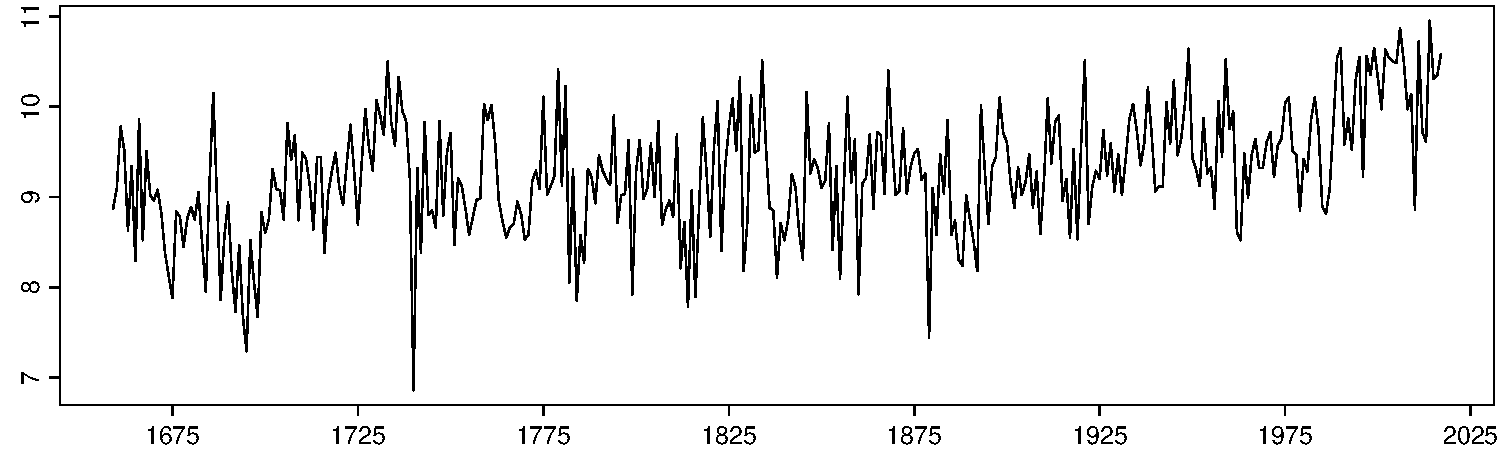
\includegraphics[width=0.9\textwidth]{Plots/temp_data.pdf}
\vspace{0.15cm}

\caption{Yearly mean temperature in Central England from 1659 to 2017 measured in $^\circ$C.}\label{temp_data}
\end{figure}


In this paper, we develop new methods to test for certain shape properties of a nonparametric time trend. We in particular construct a multiscale test which allows to identify local increases/decreases of the trend function. 
%We in particular construct a multiscale test for local increases/de\-creases of the trend function. The proposed test allows to identify, with a pre-specified statistical confidence, time regions where there is an increase/decrease in the trend. 
%identify subintervals on which the function $m$ deviates significantly from the null hypothesis of constancy. 
We develop our test in the context of the following model setting: We observe a time series $\{ Y_{t,T}: 1 \le t \le T \}$ of the form 
\begin{equation}\label{model-intro}
Y_{t,T} = m \Big( \frac{t}{T} \Big) + \varepsilon_t
\end{equation}
for $1 \le t \le T$, where $m: [0,1] \rightarrow \mathbb{R}$ is an unknown nonparametric regression function and the error terms $\varepsilon_t$ form a stationary time series process with $\ex[\varepsilon_t] = 0$. In a time series context, the design points $t/T$ represent the time points of observation and $m$ is a nonparametric time trend. As usual in nonparametric regression, we let the function $m$ depend on rescaled time $t/T$ rather than on real time $t$. A detailed description of model \eqref{model-intro} is provided in Section \ref{sec-model}.


Our multiscale test is developed step by step in Section \ref{sec-method}. Roughly speaking, the procedure can be outlined as follows: Let $H_0(u,h)$ be the hypothesis that $m$ is constant in the time window $[u-h,u+h] \subseteq [0,1]$, where $u$ is the midpoint and $2h$ the size of the window. In a first step, we set up a test statistic $\widehat{s}_T(u,h)$ for the hypothesis $H_0(u,h)$. In a second step, we aggregate the statistics $\widehat{s}_T(u,h)$ for a large number of different time windows $[u-h,u+h]$. We thereby construct a multiscale statistic which allows to test the hypothesis $H_0(u,h)$ simultaneously for many time windows $[u-h,u+h]$. In the technical part of the paper, we derive the theoretical properties of the resulting multiscale test. To do so, we come up with a proof strategy which combines strong approximation results for dependent processes with anti-concentration bounds for Gaussian random vectors. This strategy is of interest in itself and may be applied to other multiscale test problems for dependent data. As shown by our theoretical analysis, our multiscale test is a rigorous level-$\alpha$-test of the overall null hypothesis $H_0$ that $H_0(u,h)$ is simultaneously fulfilled for all time windows $[u-h,u+h]$ under consideration. Moreover, for a given significance level $\alpha \in (0,1)$, the test allows to make simultaneous confidence statements of the following form: We can claim, with statistical confidence $1-\alpha$, that there is an increase/decrease in the trend $m$ on all time windows $[u-h,u+h]$ for which the hypothesis $H_0(u,h)$ is rejected. Hence, the test allows to identify, with a pre-specified statistical confidence, time regions where the trend $m$ is increasing/decreasing. 


For independent data, multiscale tests have been developed in a variety of different contexts in recent years. In the regression context, \cite{ChaudhuriMarron1999,ChaudhuriMarron2000} introduced the so-called SiZer method which has been extended in various directions; see e.g.\ \cite{HannigMarron2006} where a refined distribution theory for SiZer is derived. \cite{HallHeckman2000} constructed a multiscale test on monotonicity of a regression function. \cite{DuembgenSpokoiny2001} developed a multiscale approach which works with additively corrected supremum statistics and derived theoretical results in the context of a continuous Gaussian white noise model. Rank-based multiscale tests for nonparametric regression were proposed in \cite{Duembgen2002} and \cite{Rohde2008}. More recently, \cite{ProkschWernerMunk2018} have constructed multiscale tests for inverse regression models. In the context of density estimation, multiscale tests have been investigated in \cite{DuembgenWalther2008}, \cite{RufibachWalther2010}, \cite{SchmidtHieber2013} and \cite{EckleBissantzDette2017} among others. 


Whereas a large number of multiscale tests for independent data have been developed in recent years, multiscale tests for dependent data are much rarer. Most notably, there are some extensions of the SiZer approach to a time series context. \cite{Rondonotti2004} and \cite{Rondonotti2007} have introduced SiZer methods for dependent data which can be used to find local increases/decreases of a trend and which may thus be regarded as an alternative to our multiscale test. However, these SiZer methods are mainly designed for data exploration rather than for rigorous statistical inference. Our multiscale method, in contrast, is a rigorous level-$\alpha$-test of the hypo\-thesis $H_0$ which allows to make simultaneous confidence statements about the time regions where the trend $m$ is increasing/decreasing. Some theoretical results for dependent SiZer methods have been derived in \cite{ParkHannigKang2009}, but only under a quite severe restriction: Only time windows $[u-h,u+h]$ with window sizes or scales $h$ are taken into account that remain bounded away from zero as the sample size $T$ grows. Scales $h$ that converge to zero as $T$ increases are excluded. This effectively means that only large time windows $[u-h,u+h]$ are taken into consideration. Our theory, in contrast, allows to simultaneously consider scales $h$ of fixed size and scales $h$ that converge to zero at various different rates. We are thus able to take into account time windows of many different sizes. \textcolor{red}{In Section \ref{subsec-method-comparison}, we compare our approach to SiZer methods in more detail.}


Our multiscale approach is also related to Wavelet-based methods: Similar to the latter, it takes into account different locations $u$ and resolution levels or scales $h$ simultaneously. However, while our multiscale approach is designed to test for local increases/decreases of a nonparametric trend, Wavelet methods are commonly used for other purposes. Among other things, they are employed for estimating/reconstructing nonparametric regression curves [see e.g.\ \cite{Donoho1995} or \cite{vonSachsMacGibbon2000}] and for change point detection [see e.g.\ \citet{ChoFryzlewicz2012}]. 


%Whereas a large number of multiscale tests for independent data have been developed in recent years, multiscale tests for dependent data are much rarer. Most notably, there are some extensions of the SiZer approach to a time series context. \cite{Rondonotti2004}, \cite{Rondonotti2007} and \cite{ParkHannigKang2009} have developed SiZer methods for dependent data which can be regarded as an alternative to our multiscale test. However, these SiZer methods are mainly designed for data exploration rather than rigorous statistical inference. Our multiscale method, in contrast, is a rigorous level-$\alpha$-test of the hypo\-thesis $H_0$, which is backed up by a complete asymptotic theory. Moreover, it allows to make simultaneous confidence statements about the time regions where the trend function $m$ is increasing/decreasing, which is not possible with the SiZer tools of \cite{Rondonotti2004}, \cite{Rondonotti2007} and \cite{ParkHannigKang2009}. Our multiscale approach is also related to Wavelet-based methods: It investigates the data on different intervals $[u-h,u+h]$. Similar to Wavelet-based procedures, it thus takes into account different locations $u$ and resolution levels $h$ simultaneously. Nevertheless, we are not aware of any Wavelet-based test for local increases/decreases of the nonparametric trend function in model \eqref{model-intro}. Wavelet methods have been used for other purposes in the literature such as estimating/reconstructing nonparametric regression functions [see e.g.\ \cite{Donoho1995} or \cite{vonSachsMacGibbon2000}] and change point detection [see e.g.\ \citet{ChoFryzlewicz2012}]. 


The test statistic of our multiscale method depends on the long-run error variance $\sigma^2 = \sum\nolimits_{\ell=-\infty}^{\infty} \cov(\varepsilon_0,\varepsilon_{\ell})$, which is usually unknown in practice. To carry out our multiscale test, we thus require an estimator of $\sigma^2$. Indeed, such an estimator is required for virtually all inferential procedures in the context of model \eqref{model-intro}. Hence, the problem of estimating $\sigma^2$ in model \eqref{model-intro} is of broader interest and has received a lot of attention in the literature; see \cite{MuellerStadtmueller1988}, \cite{Herrmann1992} and \cite{Hall2003} among many others. In Section \ref{sec-error-var}, 
%we discuss several estimators of $\sigma^2$ which are valid under different conditions on the error process $\{\varepsilon_t\}$. 
\textcolor{red}{we introduce a new difference-based estimator of $\sigma^2$ for the case that $\{ \varepsilon_t \}$ belongs to the class of AR($\infty$) processes}. This estimator improves on existing methods in several respects. 


The methodological and theoretical analysis of the paper is complemented by a simulation study in Section \ref{sec-sim} and an empirical application in Section \ref{sec-data}. In the simulation study, we examine the finite sample properties of our multiscale test and compare it to the dependent SiZer methods introduced in \cite{Rondonotti2004} and \cite{Rondonotti2007}. Moreover, we investigate the small sample performance of our estimator of $\sigma^2$ in the AR($p$) case and compare it to the estimator of \cite{Hall2003}. In Section \ref{sec-data}, we use our methods to analyse the temperature data from Figure \ref{temp_data} \textcolor{red}{as well as a sample of global temperature data}. 




\section{The model}\label{sec-model}

Before we proceed any further, we need to introduce some notation used throughout the paper. For a vector $\mathbf{v} = (v_1, \ldots, v_m)\in\reals^m$, we write $|\mathbf{v}| = \big(\sum_{i=1}^m v_i^2\big)^{1/2}$. For a random vector $\mathbf{V}$, we define it's $\mathcal{L}^q, q>1$ norm as $||\mathbf{V}||_q = \big(\ex |\mathbf{V}|^q\big)^{1/q}$. For a patricular case $q = 2$, we write $||\mathbf{V}|| := ||\mathbf{V}||_2$.

Following \cite{Wu2005}, we define the \textit{physical dependence measure} for the process $\mathbf{L}(\mathcal{F}_t)$ as the following:
\[ \delta_q(\mathbf{L}, t) = || \mathbf{L}(\mathcal{F}_t) - \mathbf{L}(\mathcal{F}_t^\prime) ||_q,
\]
where $\mathcal{F}_t  = (\ldots, \epsilon_{-1}, \epsilon_0, \epsilon_1, \ldots, \epsilon_{t-1}, \epsilon_t)$ and $\mathcal{F}_t^\prime  = (\ldots, \epsilon_{-1}, \epsilon^\prime_0, \epsilon_1, \ldots, \epsilon_{t-1}, \epsilon_t)$ is a coupled process of $\mathcal{F}_t$ with $\epsilon_0^\prime$ being an i.i.d. copy of $\epsilon_0$.

The model setting is as follows. We observe a panel of $n$ time series $\mathcal{Z}_i = \{(Y_{it}, \mathbf{X}_{it}): 1 \le t \le T \}$ of length $T$ for $1 \le i \le n$. Each time series $\mathcal{Z}_i$ satisfies the model equation \begin{equation}\label{model_full}
Y_{it} = \bm{\beta}^\top_i \mathbf{X}_{it} + m_i \Big( \frac{t}{T} \Big) + \alpha_i + \varepsilon_{it} 
\end{equation}
for $1 \le t \le T$, where $\bm{\beta}_i$ is a $d \times 1$ vector of unknown parameters, $\mathbf{X}_{it}$ is a $d\times 1$ vector of individual covariates, $m_i$ is an unknown nonparametric trend function defined on $[0,1]$, $\alpha_i$ is a (deterministic or random) intercept term and $\mathcal{E}_i = \{ \varepsilon_{it}: 1 \le t \le T \}$ is a zero-mean stationary error process. As usual in nonparametric regression, the trend functions $m_i$ in model \eqref{model_full} depend on rescaled time $t/T$ rather than on real time $t$; cp.\ \cite{Robinson1989}, \cite{Dahlhaus1997} and \cite{VogtLinton2014} for the use and some discussion of the rescaled time argument. The functions $m_i$ are only identified up to an additive constant in model \eqref{model_full}: One can reformulate the model as $Y_{it} = [m_i(t/T) + c_i] + \bm{\beta}_i^\top \mathbf{X}_{it} + [\alpha_i - c_i] + \varepsilon_{it}$, that is, one can freely shift additive constants $c_i$ between the trend $m_i(t/T)$ and the error component $\alpha_i$. In order to obtain identification, one may impose different normalization constraints on the trends $m_i$. One possibility is to normalize them such that $\int_0^1 m_i(u) du = 0$ for all $i$. In what follows, we take for granted that the trends $m_i$ satisfy this constraint. The term $\alpha_i$ can also be regarded as an additional error component. In the econometrics literature, it is commonly called a fixed effect error term. It can be interpreted as capturing unobserved characteristics of the time series $\mathcal{Z}_i$ which remain constant over time. We allow the error terms $\alpha_i$ to be dependent across $i$ in an arbitrary way. Hence, by including them in model equation \eqref{model_full}, we allow the $n$ time series $\mathcal{Z}_i$ in our panel to be correlated with each other. Whereas the terms $\alpha_i$ may be correlated, the error processes $\mathcal{E}_i$ are assumed to be independent across $i$. Technical conditions regarding the model are discussed further in this section.

Finally, note that throughout the paper, we restrict attention to the case where the number of time series $n$ in model \eqref{model_full} is fixed. Extending our theoretical results to the case where $n$ slowly grows with the sample size $T$ is a possible topic for further research.

\subsection{Assumptions}\label{subsec-model-assumptions}

Each process $\mathcal{E}_i$ is supposed to satisfy the following conditions: 

\begin{enumerate}[label=(C\arabic*),leftmargin=1.05cm]

\item \label{C-err1} For each $i$ the variables $\varepsilon_{it}$ allow for the representation $\varepsilon_{it} = G_i(\ldots,\eta_{it-1},\eta_{it})$, where $\eta_{it}$ are i.i.d.\ random variables across $t$ and $G_i: \reals^\integers \rightarrow \reals$ is a measurable function. Denote $\mathcal{J}_{it} = (\ldots,\eta_{it-2},\eta_{it-1},\eta_{it})$.

\item \label{C-err2} For all $i$ it holds that $\ex[\varepsilon_{it}] =0$ and $\| \varepsilon_{it} \|_q < \infty$ for some $q > 4$. 

\end{enumerate}

Following \cite{Wu2005}, we impose conditions on the dependence structure of the error processes $\mathcal{E}_i$ in terms of the physical dependence measure $\delta_q(G_i, t)$. In particular, we assume the following: 
\begin{enumerate}[label=(C\arabic*),leftmargin=1.05cm]
\setcounter{enumi}{2}

\item \label{C-err3} Define $\Theta_{i, t,q} = \sum\nolimits_{s \ge t} \delta_q(G_i, s)$ for $t \ge 0$. For each $i$ it holds that 
$\Theta_{i, t,q} = O ( t^{-\tau_q} (\log t)^{-A} )$,  
where $A > \frac{2}{3} (1/q + 1 + \tau_q)$ and $\tau_q = \{q^2 - 4 + (q-2) \sqrt{q^2 + 20q + 4}\} / 8q$. 

\end{enumerate}

The conditions \ref{C-err1}--\ref{C-err3} are fulfilled by a wide range of stationary processes $\mathcal{E}_i$. For a detailed discussion of these properties, see \cite{KhismatullinaVogt2018}.

Regarding the independent variables $ \mathbf{X}_{it}$, we need the following additional assumptions for each $i$:

\begin{enumerate}[label=(C\arabic*),leftmargin=1.05cm]
\setcounter{enumi}{3}

\item \label{C-reg1} The covariates $ \mathbf{X}_{it}$ allow for the representation $ \mathbf{X}_{it} = \mathbf{H}_i(\ldots,u_{it-1},u_{it})$ with $u_{it}$ being i.i.d.\ random variables and $\mathbf{H}_i := (H_{i1}, H_{i2}, \ldots, H_{id})^\top: \reals^\integers \rightarrow \reals^d$ is a measurable function such that $\mathbf{H}_i(\mathcal{U}_{it})$ is well defined. Denote $\mathcal{U}_{it} = (\ldots, u_{it-1}, u_{it})$.

\item \label{C-reg2} Let $N_i$ be the $d\times d$ matrix with $kl$-th entry $n_{i, kl}= \ex[H_{ik}(\mathcal{U}_{i0})H_{il}(\mathcal{U}_{i0})]$. We assume that the smallest eigenvalue of $N_i$ is strictly bigger than $0$.

\item \label{C-reg3} Let $\ex [\mathbf{H}_{i}(\mathcal{U}_{i0})]=\mathbf{0}$ and $||\mathbf{H}_{i}(\mathcal{U}_{it})||_4 <\infty$.
\item \label{C-reg4} $\sum_{s=0}^\infty \delta_4(\mathbf{H}_i, s)<\infty$.
\end{enumerate}

To be able to prove the main theorems in Section \ref{sec-test}, we need additional assumptions on the relationship between the covariates and the error process.

\begin{enumerate}[label=(C\arabic*),leftmargin=1.05cm]
\setcounter{enumi}{7}
\item \label{C-reg5} $\mathbf{X}_{it}$ (elementwise) and $\varepsilon_{is}$ are uncorrelated for each $t, s\in \{1, \ldots, T\}$.
\item \label{C-reg6} Let $\zeta_{i, t} = (u_{it}, \eta_{it})^\top$. Define $\mathcal{I}_{i, t} = (\ldots, \zeta_{i, t-1}, \zeta_{i, t})$ and $\mathbf{U}_i(\mathcal{I}_{i, t}) =  \mathbf{H}_i(\mathcal{U}_{it})G_i(\mathcal{J}_{it})$. Then, $\sum_{s=0}^\infty \delta_2(\mathbf{U}_i, s)<\infty$.

\end{enumerate}



\section{Testing for equality of time trends}\label{sec-test}

In this section, we adapt the multiscale method developed in \cite{KhismatullinaVogt2018} to the problem of comparison of the trend curves $m_i$ in model \eqref{model_full}.  As we will see, the proposed multiscale method does not only allow to test whether the null hypothesis is violated. It also provides information on where violations occur. More specifically, it allows to identify, with a pre-specified confidence, (i) trend functions which are different from each other and (ii) time intervals where these trend functions differ.

\subsection{Construction of the test statistic}\label{subsec-test-stat}

In what follows, we describe the construction of the test statistic that adresses the question of comparing different trend curves. More specifically, we test the null hypothesis $H_0: m_1 = m_2 = \ldots = m_n$ in model \eqref{model_full}. We assume that all the trend functions $m_i(\cdot)$ are continuosly differentiable on $[0, 1]$.

It is obvious that if $\alpha_i$ and $\bm{\beta}_i$ are known, the problem of testing for the common time trend would be greatly simplified. That is, we would test $H_0: m_1 = m_2 = \ldots = m_n$ in the model
\begin{align*}
Y_{it} - \alpha_i - \bm{\beta}_i^\top \mathbf{X}_{it} & =: Y_{it}^\circ\\
					& = m_i \Big( \frac{t}{T} \Big) + \varepsilon_{it}, 
\end{align*}
which is a standard nonparametric regression equation. The variables $Y_{it}^\circ$ are not observed since the intercept $\alpha_i$ and the coefficients $\bm{\beta}_i$ are not known. Given appropriate estimators $\widehat{\bm{\beta}}_i$ and $\widehat{\alpha}_i$, we can then consider
\begin{align*}
	\widehat{Y}_{it} := Y_{it} -\widehat{\alpha}_i - \widehat{\bm{\beta}}_i^\top \mathbf{X}_{it} =(\bm{\beta}_i - \widehat{\bm{\beta}}_i)^\top \mathbf{X}_{it} + m_i \Big( \frac{t}{T} \Big) + \big( \alpha_i - \widehat{\alpha}_i \big) + \varepsilon_{it}. 
\end{align*}

Then our unobserved variables $Y_{it}^\circ$ can be approximated by $\widehat{Y}_{it}$ and we compute our test statistic based on $\widehat{Y}_{it}$. In what follows, we assume that an estimator with the property that $\bm{\beta}_i - \widehat{\bm{\beta}}_i = O_P(T^{-1/2})$ is given.  Details on one of the possible ways to construct $\widehat{\bm{\beta}}_i$ are deferred to Section \ref{subsec-test-est}.

Given $\widehat{\bm{\beta}}_i$, consider an appropriate estimator $\widehat{\alpha}_{i}$ for the intercept $\alpha_i$ calculated by
\begin{align}\label{alpha-est}
\widehat{\alpha}_i &= \frac{1}{T}\sum_{t=1}^T \big(Y_{it} - \widehat{\bm{\beta}}_i^\top \mathbf{X}_{it}\big) = \frac{1}{T}\sum_{t=1}^T \big(\bm{\beta}_i^\top \mathbf{X}_{it} - \widehat{\bm{\beta}}_i^\top \mathbf{X}_{it} + \alpha_i + m_i(t/T) + \varepsilon_{it}\big) =\\
&= \big(\bm{\beta}_i - \widehat{\bm{\beta}}_i \big)^\top\frac{1}{T}\sum_{t=1}^T  \mathbf{X}_{it} + \alpha_i + \frac{1}{T}\sum_{i=1}^T m_i(t/T) + \frac{1}{T}\sum_{i=1}^T \varepsilon_{it}.\nonumber
\end{align}

Note that $\frac{1}{T}\sum_{i=1}^T \varepsilon_{it} = O_P(T^{-1/2})$ and $\frac{1}{T}\sum_{i=1}^T m_i(t/T) = O(T^{-1})$ due to Lipschitz continuity of $m_i$ and normalization $\int_{0}^1 m_i(u)du = 0$. Furthermore, $\frac{1}{T}\sum_{t=1}^T  \mathbf{X}_{it} = O_P(1)$ by Chebyshev's inequality and $\widehat{\bm{\beta}}_i - \bm{\beta}_i = O_P (T^{-1/2})$. Plugging all these results together in \eqref{alpha-est}, we get that $\widehat{\alpha}_i - \alpha_i = O_P(T^{-1/2})$.Thus, the unobserved variable $Y_{it}^\circ := Y_{it} - \bm{\beta}_i^\top \mathbf{X}_{it} - \alpha_i = m_i(t/T) + \varepsilon_{it}$ can be well approximated by $\widehat{Y}_{it} = Y_{it} -\widehat{\alpha}_i - \widehat{\bm{\beta}}_i^\top \mathbf{X}_{it} = Y_{it}^\circ + O_P(T^{-1/2})$.

We further let $\widehat{\sigma}_i^2$ be an estimator of the long-run error variance $\sigma_i^2 = \sum\nolimits_{\ell=-\infty}^{\infty} \cov(\varepsilon_{i0}, \varepsilon_{i\ell})$ which is computed from the constructed sample $\{ \widehat{Y}_{it}: 1 \le t \le T \}$. We thus regard $\widehat{\sigma}_i^2 = \widehat{\sigma}_i^2(\widehat{Y}_{i1},\ldots,\widehat{Y}_{iT})$ as a function of the variables $\widehat{Y}_{it}$ for $1 \le t \le T$. Throughout the section, we assume that $\widehat{\sigma}_i^2 = \sigma_i^2 + o_p(\rho_T)$ with $\rho_T = o(1/\log T)$. Details on how to construct estimators of $\sigma_i^2$ are deferred to Section \ref{sec-error-var}. 


We are now ready to introduce the multiscale statistic for testing the hypothesis $H_0: m_1 = m_2 = \ldots = m_n$. For any pair of time series $i$ and $j$, we define the kernel averages
\[ \widehat{\psi}_{ij,T}(u,h) = \sum\limits_{t=1}^T w_{t,T}(u,h)(\widehat{Y}_{it} - \widehat{Y}_{jt}), \]
where $w_{t,T}(u,h)$ are the local linear kernel weights calculated by the following formula.
\begin{equation}\label{weights}
w_{t,T}(u,h) = \frac{\Lambda_{t,T}(u,h)}{ \{\sum\nolimits_{t=1}^T \Lambda_{t,T}(u,h)^2 \}^{1/2} }, 
\end{equation}
where
\[ \Lambda_{t,T}(u,h) = K\Big(\frac{\frac{t}{T}-u}{h}\Big) \Big[ S_{T,2}(u,h) - \Big(\frac{\frac{t}{T}-u}{h}\Big) S_{T,1}(u,h) \Big], \]
$S_{T,\ell}(u,h) = (Th)^{-1} \sum\nolimits_{t=1}^T K(\frac{\frac{t}{T}-u}{h}) (\frac{\frac{t}{T}-u}{h})^\ell$ for $\ell = 0,1,2$ and $K$ is a kernel function with the following properties: 
\begin{enumerate}[label=(C\arabic*),leftmargin=1.05cm]
\setcounter{enumi}{9}
\item \label{C-ker} The kernel $K$ is non-negative, symmetric about zero and integrates to one. Moreover, it has compact support $[-1,1]$ and is Lipschitz continuous, that is, $|K(v) - K(w)| \le C |v-w|$ for any $v,w \in \reals$ and some constant $C > 0$. 
\end{enumerate} 
The kernel average $\widehat{\psi}_{ij,T}(u,h)$ can be regarded as measuring the distance between the two trend curves $m_i$ and $m_j$ on the interval $[u-h,u+h]$.

We now combine the test statistics $\widehat{\psi}_{ij, T}(u,h)$ for a wide range of different locations $u$ and bandwidths or scales $h$ in a following way:
\[ \widehat{\Psi}_{ij,T} = \max_{(u,h) \in \mathcal{G}_T} \Big\{ \Big|\frac{\widehat{\psi}_{ij,T}(u,h)}{(\widehat{\sigma}_i^2 + \widehat{\sigma}_j^2)^{1/2}}\Big| - \lambda(h) \Big\}, \] 
where $\lambda(h) = \sqrt{2 \log \{ 1/(2h) \}}$ and the set $\mathcal{G}_T$ is the set of points $(u, h)$ that are taken into
consideration. The statistic $\widehat{\Psi}_{ij,T}$ can be interpreted as a global distance measure between the two curves $m_i$ and $m_j$. Thus, the multiscale statistic $\widehat{\Psi}_{ij, T}$ simultaneously takes into account all locations $u$ and bandwidths $h$ with $(u,h) \in \mathcal{G}_T$. Throughout the paper, we suppose that $\mathcal{G}_T$ is some subset of $\mathcal{G}_T^{\text{full}} = \{ (u,h): u = t/T \text{ for some } 1 \le t \le T \text{ and } h \in [h_{\min},h_{\max}] \}$, where $h_{\min}$ and $h_{\max}$ denote some minimal and maximal bandwidth value, respectively. For our theory to work, we require the following conditions to hold:
\begin{enumerate}[label=(C\arabic*),leftmargin=1.05cm]
\setcounter{enumi}{10}

\item \label{C-grid} $|\mathcal{G}_T| = O(T^\theta)$ for some arbitrarily large but fixed constant $\theta > 0$, where $|\mathcal{G}_T|$ denotes the cardinality of $\mathcal{G}_T$. 

\item \label{C-h} $h_{\min} \gg T^{-(1-\frac{2}{q})} \log T$, that is, $h_{\min} / \{ T^{-(1-\frac{2}{q})} \log T \} \rightarrow \infty$ with $q > 4$ defined in \ref{C-err2} and $h_{\max} < 1/2$.

\end{enumerate}

We finally define the multiscale statistic for testing the null hypothesis $H_0: m_1 =m_2 = \ldots = m_n$ as
\[ \widehat{\Psi}_{n,T} = \max_{1 \le i < j \le n} \widehat{\Psi}_{ij,T}, \]
that is, we define it as the maximal distance $\widehat{\Psi}_{ij,T}$ between any pair of curves $m_i$ and $m_j$ with $i \ne j$. 

\subsection{The test procedure}\label{subsec-test-test}


Let $Z_{it}$ for $1 \le t \le T$ and $1 \le i \le n$ be independent standard normal random variables which are independent of the error terms $\varepsilon_{it}$ and the covariates $\mathbf{X}_{it}$. Denote the empirical average of the variables $Z_{i1},\ldots,Z_{iT}$ by $\bar{Z}_{i,T} = T^{-1} \sum_{t=1}^T Z_{it}$. To simplify notation, we write $\bar{Z}_i = \bar{Z}_{i,T}$ in what follows. For each $i$ and $j$, we introduce the Gaussian statistic 
\[\Phi_{ij,T} = \max_{(u,h) \in \mathcal{G}_T} \big\{ \Big|\frac{\phi_{ij,T}(u,h)}{(\widehat{\sigma}_i^2 + \widehat{\sigma}_j^2)^{1/2}}\Big| - \lambda(h) \Big\}, \] 
where $\phi_{ij,T}(u,h) = \sum\nolimits_{t=1}^T w_{t,T}(u,h) \, \big\{ \widehat{\sigma}_i (Z_{it} - \bar{Z}_i) - \widehat{\sigma}_j (Z_{jt} - \bar{Z}_j) \big\}$. Moreover, we define the statistic
\begin{align}\label{Phi-statistic}
\Phi_{n,T} = \max_{1 \le i < j \le n} \Phi_{ij,T}
\end{align}
and denote its $(1-\alpha)$-quantile by $q_{n,T}(\alpha)$. Our multiscale test of the hypothesis $H_0: m_1 = m_2 = \ldots = m_n$ is defined as follows: For a given significance level $\alpha \in (0,1)$, we reject $H_0$ if $\widehat{\Psi}_{n,T} > q_{n,T}(\alpha)$. 


\subsection{Theoretical properties of the test}\label{subsec-test-theo}


To start with, we introduce the auxiliary statistic 
\begin{align}\label{Phi-hat-statistic}
\widehat{\Phi}_{n,T} = \max_{1 \le i < j \le n} \widehat{\Phi}_{ij,T},
\end{align}
where
\[ \widehat{\Phi}_{ij,T} = \max_{(u,h) \in \mathcal{G}_T} \Big\{ \Big| \frac{\widehat{\phi}_{ij,T}(u,h)} {\{ \widehat{\sigma}_i^2 + \widehat{\sigma}_j^2 \}^{1/2}} \Big| - \lambda(h) \Big \} \]
and $\widehat{\phi}_{ij,T}(u,h) = \sum_{t=1}^T w_{t,T}(u,h) \big\{ (\varepsilon_{it} - \bar{\varepsilon}_i) + (\bm{\beta}_i - \widehat{\bm{\beta}}_i)^\top (\mathbf{X}_{it} - \bar{\mathbf{X}}_{i}) - (\varepsilon_{jt} - \bar{\varepsilon}_j) - \linebreak - (\bm{\beta}_j - \widehat{\bm{\beta}}_j)^\top (\mathbf{X}_{jt} - \bar{\mathbf{X}}_{j}) \big\}$ with $\bar{\varepsilon}_i = \bar{\varepsilon}_{i,T} = T^{-1} \sum_{t=1}^T \varepsilon_{it}$ and $ \bar{\mathbf{X}}_{i} =  \bar{\mathbf{X}}_{i, T} = T^{-1}\sum_{t=1}^T  \mathbf{X}_{it}$ respectively. Our first theoretical result characterizes the asymptotic behaviour of the statistic $\widehat{\Phi}_{n,T}$. 
\begin{theorem}\label{theo-stat-equality}
Suppose that the error processes $\mathcal{E}_i = \{ \varepsilon_{it}: 1 \le t \le T \}$ are independent across $i$ and satisfy \ref{C-err1}--\ref{C-err3} for each $i$. Moreover, let \ref{C-reg1}--\ref{C-h} be fulfilled and assume that $\widehat{\sigma}_i^2 = \sigma_i^2 + o_p(\rho_T)$ with $\rho_T = o(1/\log T)$ for each $i$. Then 
\[ \pr \big( \widehat{\Phi}_{n,T} \le q_{n,T}(\alpha) \big) = (1 - \alpha) + o(1) \]
\end{theorem}
Theorem \ref{theo-stat-equality} is the main stepping stone to derive the theoretical properties of our multiscale test. The proof of the theorem is provided in the Section \ref{subsec-appendix-stat-equality}.

%The following proposition characterizes the behaviour of our multiscale test under the null hypothesis and under local alternatives. 
%\begin{prop}\label{prop-test-equality}
%Let the conditions  of Theorem \ref{theo-stat-equality} be satisfied. 
%\begin{enumerate}[label=(\alph*),leftmargin=0.75cm]
%\item Under the null hypothesis $H_0: m_1 = m_2 = \ldots = m_n$, it holds that 
%\[ \pr \big( \widehat{\Psi}_{n,T} \le q_{n,T}(\alpha) \big) = (1 - \alpha) + o(1). \]
%\item Let $m_i = m_{i,T}$ be a Lipschitz continuous function with $\int_0^1 m_{i,T}(w) dw = 0$ for any $i$. In particular, suppose that $|m_{i,T}(v) - m_{i,T}(w)| \le L |v - w|$ for all $v,w \in [0,1]$ and some fixed constant $L < \infty$ which does not depend on $T$. Moreover, assume that for some pair of indices $i$ and $j$, the functions $m_{i,T}$ and $m_{j,T}$ have the following property: There exists $(u,h) \in \mathcal{G}_T$ with $[u-h,u+h] \subseteq [0,1]$ such that $m_{i,T}(w) - m_{j,T}(w) \ge c_T \sqrt{\log T/(Th)}$ for all $w \in [u-h,u+h]$ or $m_{j,T}(w) - m_{i,T}(w) \ge c_T \sqrt{\log T/(Th)}$ for all $w \in [u-h,u+h]$, where $\{c_T\}$ is any sequence of positive numbers with $c_T \rightarrow \infty$. Then 
%\[ \pr \big( \widehat{\Psi}_{n,T} \le q_{n,T}(\alpha) \big) = o(1). \]
%\end{enumerate}
%\end{prop}

\subsection{Estimation of the parameters $\bm{\beta}_i$}\label{subsec-test-est}

We now focus on finding an appropriate estimator $\widehat{\bm{\beta}}_i$ of $\bm{\beta}_i$. For that purpose, for each $i$ we consider the time series $\{\Delta Y_{it}: 2 \leq t \leq T\}$ of the differences $\Delta Y_{it} = Y_{it} - Y_{i t-1}$. We then have
\begin{align*}
	\Delta Y_{it} = Y_{it} - Y_{i t-1} =\bm{\beta}_i^\top \Delta \mathbf{X}_{it} + \bigg(m_i \Big( \frac{t}{T} \Big) - m_i \Big(\frac{t-1}{T}\Big)\bigg) + \Delta \varepsilon_{it},
\end{align*}
where $\Delta  \mathbf{X}_{it} =  \mathbf{X}_{it} -  \mathbf{X}_{it-1}$ and $ \Delta \varepsilon_{it} = \varepsilon_{it} - \varepsilon_{i t-1}$. Since $m_i(\cdot)$ is Lipschitz, we can use the fact that $ \big|m_i \big( \frac{t}{T} \big) - m_i \big(\frac{t-1}{T}\big) \big| = O\big(\frac{1}{T}\big)$ and rewrite 
\begin{align}\label{model_with_regs}
	\Delta Y_{it} = \bm{\beta}_i^\top \Delta \mathbf{X}_{it} + \Delta \varepsilon_{it} + O\Big(\frac{1}{T}\Big).
\end{align}

In particular, for each $i$ we employ the least squares estimation method to estimate $\bm{\beta}_i$ in \eqref{model_with_regs}, treating $\Delta \mathbf{X}_{it}$ as the regressors and $\Delta Y_{it}$ as the response variable. That is, we propose the following differencing estimator:
\begin{align}\label{dif-est}
\widehat{\bm{\beta}}_i = \Big( \sum_{t=2}^T \Delta \mathbf{X}_{it} \Delta \mathbf{X}_{it}^\top \Big)^{-1} \sum_{t=2}^T \Delta \mathbf{X}_{it} \Delta Y_{it}
\end{align}

Then the asymptotic consistency for this differencing estimator is given by the following theorem:

\begin{theorem}\label{theo-regs}
Under Assumptions \ref{C-err1} - \ref{C-reg6}, we have
\[\bm{\beta}_i - \widehat{\bm{\beta}}_i  = O_P \Big(\frac{1}{\sqrt{T}}\Big),
\]
where $\widehat{\bm{\beta}}_i$ is the differencing estimator given by \eqref{dif-est}.
\end{theorem}


%\item Let $m_i = m_{i,T}$ be a Lipschitz continuous function with $\int_0^1 m_{i,T}(w) dw = 0$ for any $i$. In particular, suppose that $|m_{i,T}(v) - m_{i,T}(w)| \le L |v - w|$ for all $v,w \in [0,1]$ and some fixed constant $L < \infty$ which does not depend on $T$. Moreover, assume that for some pair of indices $i$ and $j$, the functions $m_{i,T}$ and $m_{j,T}$ have the following property: There exists $(u,h) \in \mathcal{G}_T$ with $[u-h,u+h] \subseteq [0,1]$ such that $m_{i,T}(w) - m_{j,T}(w) \ge c_T \sqrt{\log T/(Th)}$ for all $w \in [u-h,u+h]$ or $m_{j,T}(w) - m_{i,T}(w) \ge c_T \sqrt{\log T/(Th)}$ for all $w \in [u-h,u+h]$, where $\{c_T\}$ is any sequence of positive numbers with $c_T \rightarrow \infty$. Then 
%\[ \pr \big( \widehat{\Psi}_{n,T}^\prime \le q_{n,T}^\prime(\alpha) \big) = o(1). \]






%\section{Clustering}
%\subsection{Clustering of time trends}\label{subsec-test-equality-clustering}
%
%
%Consider a situation in which the null hypothesis $H_0: m_1 = m_2 = \ldots = m_n$ is violated. Even though some of the trend functions are different in this case, part of them may still be the same. Put differently, there may be groups of time series which have the same time trend. Formally speaking, we define a group structure as follows: There exist sets or groups of time series $G_1,\ldots,G_N$ with $N \le n$ and $\{1,\ldots,n\} = \mathbin{\dot{\bigcup}}_{\ell=1}^{N} G_\ell$ such that for each $1 \le \ell \le N$,
%\[ m_i = g_\ell \quad \text{for all } i \in G_\ell, \]
%where $g_\ell$ are group-specific trend functions. Hence, the time series which belong to the group $G_\ell$ all have the same time trend $g_\ell$. Throughout the section, we suppose that the group-specific trend functions $g_\ell$ have the following properties: For each $\ell$, $g_\ell = g_{\ell,T}$ is a Lipschitz continuous function with $\int_0^1 g_{\ell,T}(w) dw = 0$. In particular, it holds that $|g_{\ell,T}(v) - g_{\ell,T}(w)| \le L |v-w|$ for all $v,w \in [0,1]$ and some constant $L < \infty$ that does not depend on $T$. Moreover, for any $\ell \ne \ell^\prime$, the trends $g_{\ell,T}$ and $g_{\ell^\prime,T}$ are assumed to differ in the following sense: There exists $(u,h) \in \mathcal{G}_T$ with $[u-h,u+h] \subseteq [0,1]$ such that $g_{\ell,T}(w) - g_{\ell^\prime,T}(w) \ge c_T \sqrt{\log T/(Th)}$ for all $w \in [u-h,u+h]$ or $g_{\ell^\prime,T}(w) - g_{\ell,T}(w) \ge c_T \sqrt{\log T/(Th)}$ for all $w \in [u-h,u+h]$, where $0 < c_T \rightarrow \infty$.
%
%
%In many applications, it is natural to suppose that there is a group structure in the data. In this case, a particular interest lies in estimating the unknown groups from the data at hand. In what follows, we combine our multiscale methods with a clustering algorithm to achieve this. More specifically, we use the multiscale statistics $\widehat{\Psi}_{ij,T}$ as distance measures which are fed into a hierarchical clustering algorithm. To describe the algorithm, we first need to introduce the notion of a dissimilarity measure: Let $S \subseteq \{1,\ldots,n\}$ and $S^\prime \subseteq \{1,\ldots,n\}$ be two sets of time series from our sample. We define a dissimilarity measure between $S$ and $S^\prime$ by setting 
%\begin{equation}\label{dissimilarity}
%\widehat{\Delta}(S,S^\prime) = \max_{\substack{i \in S, \\ j \in S^\prime}} \widehat{\Psi}_{ij,T}. 
%\end{equation}
%This is commonly called a complete linkage measure of dissimilarity. Alternatively, we may work with an average or a single linkage measure. We now combine the dissimilarity measure $\widehat{\Delta}$ with a hierarchical agglomerative clustering (HAC) algorithm which proceeds as follows: 
%\vspace{10pt}
%
%\noindent \textit{Step $0$ (Initialization):} Let $\widehat{G}_i^{[0]} = \{ i \}$ denote the $i$-th singleton cluster for $1 \le i \le n$ and define $\{\widehat{G}_1^{[0]},\ldots,\widehat{G}_n^{[0]} \}$ to be the initial partition of time series into clusters. 
%\vspace{5pt}
%
%\noindent \textit{Step $r$ (Iteration):} Let $\widehat{G}_1^{[r-1]},\ldots,\widehat{G}_{n-(r-1)}^{[r-1]}$ be the $n-(r-1)$ clusters from the previous step. Determine the pair of clusters $\widehat{G}_{\ell}^{[r-1]}$ and $\widehat{G}_{{\ell}^\prime}^{[r-1]}$ for which 
%
%\[ \widehat{\Delta}(\widehat{G}_{\ell}^{[r-1]},\widehat{G}_{{\ell}^\prime}^{[r-1]}) = \min_{1 \le k < k^\prime \le n-(r-1)} \widehat{\Delta}(\widehat{G}_{k}^{[r-1]},\widehat{G}_{k^\prime}^{[r-1]}) \]  
%and merge them into a new cluster. 
%\vspace{10pt}
%
%\noindent Iterating this procedure for $r = 1,\ldots,n-1$ yields a tree of nested partitions $\{\widehat{G}_1^{[r]},\ldots$ $\ldots,\widehat{G}_{n-r}^{[r]}\}$, which can be graphically represented by a dendrogram. Roughly speaking, the HAC algorithm merges the $n$ singleton clusters $\widehat{G}_i^{[0]} = \{ i \}$ step by step until we end up with the cluster $\{1,\ldots,n\}$. In each step of the algorithm, the closest two clusters are merged, where the distance between clusters is measured in terms of the dissimilarity $\widehat{\Delta}$. We refer the reader to Section 14.3.12 in \cite{HastieTibshiraniFriedman2009} for an overview of hierarchical clustering methods. 
%
%
%When the number of groups $N$ is known, we estimate the group structure $\{G_1,\ldots, G_N\}$ by the $N$-partition $\{\widehat{G}_1^{[n-N]},\ldots,\widehat{G}_{N}^{[n-N]}\}$ produced by the HAC algorithm. When $N$ is unknown, we estimate it by the $\widehat{N}$-partition $\{\widehat{G}_1^{[n-\widehat{N}]},\ldots,\widehat{G}_{\widehat{N}}^{[n-\widehat{N}]}\}$, where $\widehat{N}$ is an estimator of $N$. The latter is defined as 
%\[ \widehat{N} = \min \Big\{ r = 1,2,\ldots \Big| \max_{1 \le \ell \le r} \widehat{\Delta} \big( \widehat{G}_\ell^{[n-r]} \big) \le q_{n,T}(\alpha) \Big\}, \]
%where we write $\widehat{\Delta}(S) = \widehat{\Delta}(S,S)$ for short and $q_{n,T}(\alpha)$ is the $(1-\alpha)$-quantile of $\Phi_{n,T}$ defined in Section \ref{subsec-test-equality-test}. 
%
%
%\newpage
%The following proposition summarizes the theoretical properties of the estimators $\widehat{N}$ and $\{ \widehat{G}_1,\ldots,\widehat{G}_{\widehat{N}} \}$, where we use the shorthand $\widehat{G}_\ell = \widehat{G}_\ell^{[n-\widehat{N}]}$ for $1 \le \ell \le \widehat{N}$. 
%\begin{prop}\label{prop-clustering-1}
%Let the conditions of Theorem \ref{theo-stat-equality} be satisfied. Then 
%\[ \pr \Big( \big\{ \widehat{G}_1,\ldots,\widehat{G}_{\widehat{N}} \big\} = \{ G_1,\ldots,G_N \} \Big) \ge (1-\alpha) + o(1) \]
%and 
%\[ \pr \big( \widehat{N} = N \big) \ge (1-\alpha) + o(1). \]
%\end{prop}
%This result allows us to make statistical confidence statements about the estimated clusters $\{ \widehat{G}_1,\ldots,\widehat{G}_{\widehat{N}} \}$ and their number $\widehat{N}$. In particular, we can claim with asymptotic confidence $\ge 1 - \alpha$ that the estimated group structure is identical to the true group structure. Note that it is possible to let the significance level $\alpha$ depend on the sample size $T$ in Proposition \ref{prop-clustering-1}. In particular, we can allow $\alpha = \alpha_T$ to converge slowly to zero as $T \rightarrow \infty$, in which case we obtain that $\pr ( \{ \widehat{G}_1,\ldots,\widehat{G}_{\widehat{N}} \} = \{ G_1,\ldots,G_N \} ) \rightarrow 1$ and $\pr ( \widehat{N} = N ) \rightarrow 1$. The proof of Proposition \ref{prop-clustering-1} can be found in the Supplementary Material.   
%
%
%Our multiscale methods do not only allow us to compute estimators of the unknown groups $G_1,\ldots,G_N$. They also provide information on the locations where two group-specific trend functions $g_\ell$ and $g_{\ell^\prime}$ differ from each other. To turn this claim into a mathematically precise statement, we need to introduce some notation. First of all, note that the indexing of the estimators $\widehat{G}_1,\ldots,\widehat{G}_{\widehat{N}}$ is completely arbitrary. We could, for example, change the indexing according to the rule $\ell \mapsto \widehat{N} - \ell + 1$. In what follows, we suppose that the estimated groups are indexed such that $P( \widehat{G}_\ell = G_\ell \text{ for all } \ell ) \ge (1-\alpha) + o(1)$. Theorem \ref{prop-clustering-1} implies that this is possible without loss of generality. Keeping this convention in mind, we define the sets 
%\[ \mathcal{A}_{n,T}(\ell,\ell^\prime) = \Big\{ (u,h) \in \mathcal{G}_T: \Big| \frac{\widehat{\psi}_{ij,T}(u,h)}{(\widehat{\sigma}_i^2 + \widehat{\sigma}_j^2)^{1/2}} \Big| > q_{n,T}(\alpha) + \lambda(h) \text{ for some } i \in \widehat{G}_\ell, j \in \widehat{G}_{\ell^\prime} \Big\} \] 
%and  
%\[ \Pi_{n,T}(\ell,\ell^\prime) = \big\{ I_{u,h} = [u-h,u+h]: (u,h) \in \mathcal{A}_{n,T}(\ell,\ell^\prime) \big\} \]
%for $1 \le \ell < \ell^\prime \le \widehat{N}$. An interval $I_{u,h}$ is contained in $\Pi_{n,T}(\ell,\ell^\prime)$ if our multiscale test indicates a significant difference between the trends $m_i$ and $m_j$ on the interval $I_{u,h}$ for some $i \in \widehat{G}_\ell$ and $j \in \widehat{G}_{\ell^\prime}$. Put differently,  $I_{u,h} \in \Pi_{n,T}(\ell,\ell^\prime)$ if the test suggests a significant difference between the trends of the $\ell$-th and the $\ell^\prime$-th group on the interval $I_{u,h}$. We further let
%\[ E_{n,T}(\ell,\ell^\prime) = \Big\{ \forall I_{u,h} \in \Pi_{n,T}(\ell,\ell^\prime): g_\ell(v) \ne g_{\ell^\prime}(v) \text{ for some } v \in I_{u,h} = [u-h,u+h] \Big\} \]
%be the event that the group-specific time trends $g_\ell$ and $g_{\ell^\prime}$ differ on all intervals $I_{u,h} \in \Pi_{n,T}(\ell,\ell^\prime)$. With this notation at hand, we can make the following formal statement whose proof is given in the Supplementary Material.
%\begin{prop}\label{prop-clustering-2}
%Under the conditions of Theorem \ref{theo-stat-equality}, the event 
%\[ E_{n,T} = \Big\{ \bigcap_{1 \le \ell < \ell^\prime \le \widehat{N}} E_{n,T}(\ell,\ell^\prime) \Big\} \cap \Big\{ \widehat{N} = N \text{ and } \widehat{G}_\ell = G_\ell \text{ for all } \ell \Big\} \]
%asymptotically occurs with probability $\ge 1-\alpha$, that is, 
%\[ \pr \big( E_{n,T} \big) \ge (1 - \alpha) + o(1). \]
%\end{prop}
%The statement of Proposition \ref{prop-clustering-2} remains to hold true when the sets of intervals $\Pi_{n,T}(\ell,\ell^\prime)$ are replaced by the corresponding sets of minimal intervals. According to Proposition \ref{prop-clustering-2}, the sets $\Pi_{n,T}(\ell,\ell^\prime)$ allow us to locate, with a pre-specified confidence, time regions where the group-specific trend functions $g_\ell$ and $g_{\ell^\prime}$ differ from each other. In particular, we can claim with asymptotic confidence $\ge 1 - \alpha$ that the trend functions $g_\ell$ and $g_{\ell^\prime}$ differ on all intervals $I_{u,h} \in \Pi_{n,T}(\ell,\ell^\prime)$.


%\newpage
\bibliographystyle{ims}
{\small
\setlength{\bibsep}{0.55em}
\nobibliography{bibliography}}

\section{Appendix}\label{sec-appendix}

\subsection{Proof of Theorem \ref{theo-stat-equality}}\label{subsec-appendix-stat-equaility}


In this section, we prove the theoretical results from Section \ref{sec-test}. We use the following notation: The symbol $C$ denotes a universal real constant which may take a different value on each occurrence. For $a,b \in \reals$, we write $a_+ = \max \{0,a\}$ and $a \vee b = \max\{a,b\}$. For any set $A$, the symbol $|A|$ denotes the cardinality of $A$. The notation $X \stackrel{\mathcal{D}}{=} Y$ means that the two random variables $X$ and $Y$ have the same distribution. Finally, $f_0(\cdot)$ and $F_0(\cdot)$ denote the density and the distribution function of the standard normal distribution, respectively.

\subsection*{Introducing additional intermediate statistic}

The auxiliary statistic $\widehat{\Phi}_{n,T}$ defined in Section \ref{subsec-test-theo} (which is basically the version of the main statistic $\widehat{\Psi}_{n,T}$ under the null hypothesis) heavily depends on the known covariates $\mathbf{X}_{it}$, whereas the Gaussian version $\Phi_{n,T}$ does not. This is the reason why we need to introduce additional intermediate test statistic that connects  $\widehat{\Phi}_{n,T}$ and $\Phi_{n,T}$. Thus, for each $i$ and $j$, consider the following kernel averages:
\[\doublehat{\phi}_{ij,T}(u,h) = \sum_{t=1}^T w_{t,T}(u,h) \big\{ (\varepsilon_{it} - \bar{\varepsilon}_i) - (\varepsilon_{jt} - \bar{\varepsilon}_j)  \big\}. \]
The intermediate statistic is then defined as 
\begin{align}\label{Phi-doublehat-statistic}
\doublehattwo{\Phi}_{n,T} &= \max_{1 \le i < j \le n} \doublehattwo{\Phi}_{ij,T}\quad  \text{with} \\
\doublehattwo{\Phi}_{ij,T} &= \max_{(u,h) \in \mathcal{G}_T} \big\{ \Big|\frac{\doublehat{\phi}_{ij,T}(u,h)}{(\widehat{\sigma}_i^2 + \widehat{\sigma}_j^2)^{1/2}}\Big| - \lambda(h) \Big\}.\nonumber
\end{align}
This statistic can thus be regarded as an approximation of the statistic $\widehat{\Phi}_{n,T}$. Heuristically, the kernel averages $\doublehat{\phi}_{ij,T}(u,h)$
are close to the kernel averages $\widehat{\phi}_{ij,T}(u,h)$ because of the properties of our estimators $\widehat{\bf{\beta}}_i$ and assumptions on $\mathbf{X}_{it}$ but we will prove it later in this Section.


\subsection*{Auxiliary results using strong approximation theory}

The main purpose of this section is to prove that there is a version of the multiscale statistic $\doublehattwo{\Phi}_{n,T}$ defined in \eqref{Phi-doublehat-statistic} which is close to a Gaussian statistic whose distribution is known. More specifically, we prove the following result. 

\begin{propA}\label{propA-strong-approx-equality}
Under the conditions of Theorem \ref{theo-stat-equality}, there exist statistics $\widetilde{\Phi}_{n,T}$ for $T = 1,2,\ldots$ with the following two properties: (i) $\widetilde{\Phi}_{n, T}$ has the same distribution as $\doublehattwo{\Phi}_{n, T}$ for any $T$, and (ii)
\begin{align*}
\big| \widetilde{\Phi}_{n, T} - \Phi_{n,T} \big| = o_p \Big( \frac{T^{1/q}}{\sqrt{T h_{\min}}} &+ \frac{\rho_T}{\sqrt{h_{\min}}}\sqrt{\log T} \Big),
\end{align*}
where $\Phi_{n,T}$ is a Gaussian statistic as defined in \eqref{Phi-statistic}. 
\end{propA}
\begin{proof}[\textnormal{\textbf{Proof of Proposition \ref{propA-strong-approx-equality}}}] 
For the proof, we draw on strong approximation theory for each stationary process $\mathcal{E}_i = \{\varepsilon_{it}: 1 \leq t \leq T\}$ that fulfill the conditions \ref{C-err1}--\ref{C-err3}. By Theorem 2.1 and Corollary 2.1 in \cite{BerkesLiuWu2014}, the following strong approximation result holds true: On a richer probability space, there exist a standard Brownian motion $\mathbb{B}$ and a sequence $\{ \widetilde{\varepsilon}_{t}: t \in \naturals \}$ such that $[\widetilde{\varepsilon}_{1},\ldots,\widetilde{\varepsilon}_{T}] \stackrel{\mathcal{D}}{=} [\varepsilon_{1},\ldots,\varepsilon_{T}]$ for each $T$ and 
\begin{equation}\label{eq-strongapprox-dep}
\max_{1 \le t \le T} \Big| \sum\limits_{s=1}^t \widetilde{\varepsilon}_{s} - \sigma \mathbb{B}(t) \Big| = o\big( T^{1/q} \big) \quad \text{a.s.},  
\end{equation}
where $\sigma^2 = \sum_{k \in \integers} \cov(\varepsilon_{0}, \varepsilon_{k})$ denotes the long-run error variance.

We apply this result for each stationary process $\mathcal{E}_i = \{\varepsilon_{it}: 1 \leq t \leq T\}$ separately. In order to do this, we define 
\begin{align}\label{Phi-tilde-statistic}
\widetilde{\Phi}_{n,T} = \max_{1 \le i < j \le n} \widetilde{\Phi}_{ij,T},
\end{align}
where
\[ \widetilde{\Phi}_{ij, T} = \max_{(u,h) \in \mathcal{G}_T} \Big\{ \Big|\frac{\widetilde{\phi}_{ij, T}(u,h)}{\{\widetilde{\sigma}_i^2 + \widetilde{\sigma}_j^2 \}^{1/2}} \Big| - \lambda(h) \Big\}, \]
where $\widetilde{\phi}_{ij, T}(u,h) = \sum\nolimits_{t=1}^T w_{t,T}(u,h) \big\{ (\widetilde{\varepsilon}_{it} - \bar{\widetilde{\varepsilon}}_i)  - (\widetilde{\varepsilon}_{jt} - \bar{\widetilde{\varepsilon}}_j)\big\}$ and $\widetilde{\sigma}^2_i$ are the same estimators as $\widehat{\sigma}^2_i$ with $\widehat{Y}_{it} = (\bm{\beta}_i - \widehat{\bm{\beta}}_i)^\top \mathbf{X}_{it} + m_i ( t/T) + \big( \alpha_i - \widehat{\alpha}_i \big) + \varepsilon_{it}$
replaced by $\widetilde{Y}_{it} = \linebreak = (\bm{\beta}_i - \widehat{\bm{\beta}}_i)^\top \mathbf{X}_{it} + m_i(t/T) + \big( \alpha_i - \widehat{\alpha}_i \big) + \widetilde{\varepsilon}_{it}$  for $1 \le t \le T$. In addition, we let
\begin{align*}
\Phi_{n, T} & = \max_{1\leq i < j \leq n} \Phi_{ij, T}= \max_{1\leq i < j \leq n} \max_{(u,h) \in \mathcal{G}_T} \Big\{ \Big|\frac{\phi_{ij, T}(u,h)}{\{\widehat{\sigma}_i^2 + \widehat{\sigma}_j^2 \}^{1/2}}\Big| - \lambda(h) \Big\} \\
\Phi_{n, T}^{\diamond} & =\max_{1\leq i < j \leq n} \Phi_{ij, T}^{\diamond} = \max_{1\leq i< j \leq n}\max_{(u,h) \in \mathcal{G}_T} \Big\{ \Big|\frac{\phi_{ij, T}(u,h)}{\{\widetilde{\sigma}_i^2 + \widetilde{\sigma}_j^2 \}^{1/2}}\Big| - \lambda(h) \Big\} 
\end{align*}
with $$\phi_{ij, T}(u,h) = \sum\nolimits_{t=1}^T w_{t,T}(u,h) \big\{ \widehat{\sigma}_i (Z_{it} - \bar{Z}_i) - \widehat{\sigma}_j (Z_{jt} - \bar{Z}_j) \big\}$$ and $Z_{it} = \mathbb{B}_i(t) - \mathbb{B}_i(t-1)$. With this notation, we can write 
\begin{equation}\label{eq-strongapprox-bound1}
\big| \widetilde{\Phi}_{n, T} - \Phi_{n, T} \big| \le \big| \widetilde{\Phi}_{n, T} - \Phi_{n, T}^{\diamond} \big| + \big| \Phi_{n, T}^{\diamond} - \Phi_{n, T} \big|. 
\end{equation}
First consider $|\widetilde{\Phi}_{n, T} - \Phi_{n, T}^{\diamond}|$. Straightforward calculations yield that 
\begin{align}\label{eq-strongapprox-bound2}
\big| \widetilde{\Phi}_{n, T} - \Phi_{n, T}^{\diamond} \big| \le \{\widetilde{\sigma}_i^2 + \widetilde{\sigma}_j^2 \}^{-1/2} \max_{1\le i < j \le n} \max_{(u,h) \in \mathcal{G}_T} \big| \widetilde{\phi}_{ij, T}(u,h) - \phi_{ij, T}(u,h) \big|.
\end{align}
Using summation by parts,
($\sum_{i=1}^n a_i b_i = \sum_{i=1}^{n-1} A_i (b_i - b_{i+1}) + A_n b_n$ with $A_j = \sum_{j=1}^i a_j$) 
we further obtain that 
\begin{align*}
\big| \widetilde{\phi}_{ij, T}(u,h) &- \phi_{ij, T}(u,h) \big| = \\
=&\bigg|\sum_{t=1}^T w_{t,T}(u,h) \big\{ (\widetilde{\varepsilon}_{it} - \bar{\widetilde{\varepsilon}}_i) - (\widetilde{\varepsilon}_{jt} - \bar{\widetilde{\varepsilon}}_j) -\widehat{\sigma}_i (Z_{it} - \bar{Z}_i) + \widehat{\sigma}_j (Z_{jt} - \bar{Z}_j) \big\}\bigg| = \\
=&\Big|\sum_{t=1}^{T-1} A_{ij, t} \big(w_{t,T}(u,h) -w_{t+1,T}(u,h)\big) + A_{ij, T} w_{T,T}(u,h)\Big|,
\end{align*}
where 
\begin{align*}
A_{ij, t} = \sum_{s=1}^t \big\{ (\widetilde{\varepsilon}_{is} - \bar{\widetilde{\varepsilon}}_i)  - (\widetilde{\varepsilon}_{js} - \bar{\widetilde{\varepsilon}}_j) - \widehat{\sigma}_i (Z_{it} - \bar{Z}_i) + \widehat{\sigma}_j (Z_{jt} - \bar{Z}_j) \big\}.
\end{align*}
Note that by construction $A_{ij, T} = 0$ for all pairs $(i, j)$. Denoting 
\[ W_T(u,h) = \sum\limits_{t=1}^{T-1} |w_{t+1,T}(u,h) - w_{t,T}(u,h)|,\]
we have 
\begin{align}\label{eq-strongapprox-bound3}
\big| \widetilde{\phi}_{ij, T}(u,h) - \phi_{ij, T}(u,h) \big| =& \Big|\sum_{t=1}^{T-1} A_{ij, t} \big(w_{t,T}(u,h) -w_{t+1,T}(u,h)\big)\Big|\le W_T(u, h)\max_{1 \le t \le T} |A_{ij, t}|.
\end{align}
Now consider $\max_{1 \le t \le T} |A_{ij, t}|$:
\begin{align*}
\max_{1 \le t \le T} |A_{ij, t}|  \le & \max_{1 \le t \le T} \Big| \sum\limits_{s=1}^t (\widetilde{\varepsilon}_{is} - \bar{\widetilde{\varepsilon}}_{i}) - \widehat{\sigma}_i \sum\limits_{s=1}^t \big\{ Z_{is} - \bar{Z_i} \big\} \Big| + \max_{1 \le t \le T} \Big| \sum\limits_{s=1}^t (\widetilde{\varepsilon}_{js} - \bar{\widetilde{\varepsilon}}_{j}) - \widehat{\sigma}_j \sum\limits_{s=1}^t \big\{ Z_{js} - \bar{Z_j} \big\} \Big| \le \\
\le & \max_{1 \le t \le T} \Big| \sum\limits_{s=1}^t \widetilde{\varepsilon}_{is} - \widehat{\sigma}_i \sum\limits_{s=1}^t Z_{is} \Big| + \max_{1 \le t \le T} \Big| t (\bar{\widetilde{\varepsilon}}_{i} - \widehat{\sigma}_i \bar{Z_i}) \Big|+\\
& + \max_{1 \le t \le T} \Big| \sum\limits_{s=1}^t \widetilde{\varepsilon}_{js} - \widehat{\sigma}_j \sum\limits_{s=1}^t Z_{js} \Big| + \max_{1 \le t \le T} \Big| t (\bar{\widetilde{\varepsilon}}_{j} -\widehat{\sigma}_j \bar{Z_j}) \Big|= \\
= & \max_{1 \le t \le T} \Big| \sum\limits_{s=1}^t \widetilde{\varepsilon}_{is} - \widehat{\sigma}_i \sum\limits_{s=1}^t Z_{is} \Big| + T \Big| \frac{1}{T}\Big(\sum\limits_{s=1}^T \widetilde{\varepsilon}_{is} - \widehat{\sigma}_i \sum\limits_{s=1}^T Z_{is}\Big)\Big|+\\
& + \max_{1 \le t \le T} \Big| \sum\limits_{s=1}^t \widetilde{\varepsilon}_{js} - \widehat{\sigma}_j \sum\limits_{s=1}^t Z_{js} \Big| +  T \Big| \frac{1}{T}\Big(\sum\limits_{s=1}^T \widetilde{\varepsilon}_{js} -\widehat{\sigma}_j \sum\limits_{s=1}^T  Z_{js}\Big)\Big| \le \\
\le & 2 \max_{1 \le t \le T} \Big| \sum\limits_{s=1}^t \widetilde{\varepsilon}_{is} -\widehat{\sigma}_i \sum\limits_{s=1}^t Z_{is} \Big| + 2 \max_{1 \le t \le T} \Big| \sum\limits_{s=1}^t \widetilde{\varepsilon}_{js} -\widehat{\sigma}_j \sum\limits_{s=1}^t Z_{js} \Big| =\\
= & 2 \max_{1 \le t \le T} \Big| \sum\limits_{s=1}^t \widetilde{\varepsilon}_{is} - \widehat{\sigma}_i \sum\limits_{s=1}^t \big(\mathbb{B}_{i}(s) - \mathbb{B}_{i}(s-1) \big) \Big| +\\
& +  2 \max_{1 \le t \le T} \Big| \sum\limits_{s=1}^t \widetilde{\varepsilon}_{js} -\widehat{\sigma}_j \sum\limits_{s=1}^t \big(\mathbb{B}_{j}(s) - \mathbb{B}_{j}(s-1) \big) \Big| =\\
= & 2 \max_{1 \le t \le T} \Big| \sum\limits_{s=1}^t \widetilde{\varepsilon}_{is} - \widehat{\sigma}_i \mathbb{B}_{i}(t) \Big| + 2 \max_{1 \le t \le T} \Big| \sum\limits_{s=1}^t \widetilde{\varepsilon}_{js} - \widehat{\sigma}_j \mathbb{B}_{j}(t) \Big| \le\\
\le & 2 \max_{1 \le t \le T} \Big| \sum\limits_{s=1}^t \widetilde{\varepsilon}_{is} - \sigma_i \mathbb{B}_{i}(t) \Big| + 2 \max_{1 \le t \le T}\Big|\sigma_i \mathbb{B}_{i}(t) - \widehat{\sigma}_i \mathbb{B}_{i}(t)  \Big| +\\
&+ 2 \max_{1 \le t \le T} \Big| \sum\limits_{s=1}^t \widetilde{\varepsilon}_{js} - \sigma_j \mathbb{B}_{j}(t) \Big| + 2 \max_{1 \le t \le T} \Big| \sigma_j \mathbb{B}_{j}(t) - \widehat{\sigma}_j \mathbb{B}_{j}(t) \Big|
\end{align*}
Note that for all $1 \le i \le n$ we have $\widehat{\sigma}_i^2 - \sigma_i^2 = o_P(\rho_T)$ which leads to $\widehat{\sigma}_i - \sigma_i = o_P(\rho_T)$. Furthermore, regarding the standard Brownian motion $\mathbb{B}_{i}(t)$ as a sum of standard normal random variables, we get the following result:
\begin{align*}
 \max_{1 \le t \le T} |\mathbb{B}_{i}(t) | &=  \max_{1 \le t \le T}\big|\sum_{s=1}^t Z_{is} \big| = \max_{1 \le t \le T}\Big|\sqrt{t} \frac{1}{\sqrt{t}}\sum_{s=1}^t Z_{is} \Big| \le \\
 &\le \max_{1 \le t \le T}\sqrt{t}  \max_{1 \le t \le T}\Big| \frac{1}{\sqrt{t}}\sum_{s=1}^t Z_{is} \Big| = \sqrt{T}  \max_{1 \le t \le T}\Big| \frac{1}{\sqrt{t}}\sum_{s=1}^t Z_{is} \Big| = O_P(\sqrt{T \log T}),
\end{align*}
where we used the bound for the maximum of $T$ standard normal random variables and the fact that for each $t$, $1\le t \le T$, $ \frac{1}{\sqrt{t}}\sum_{s=1}^t Z_{is}$ is a standard normal random variable.

Therefore, applying the strong approximation result \eqref{eq-strongapprox-dep}, we can infer that
\begin{align}\label{max_At}
\max_{1 \le t \le T} |A_{ij, t}|  \le & 2 \max_{1 \le t \le T} \Big| \sum\limits_{s=1}^t \widetilde{\varepsilon}_{is} - \sigma_i \mathbb{B}_{i}(t) \Big| + 2\big|\sigma_i - \widehat{\sigma}_i\big|  \max_{1 \le t \le T}\big|\mathbb{B}_{i}(t) \big| +\nonumber\\
&+ 2 \max_{1 \le t \le T} \Big| \sum\limits_{s=1}^t \widetilde{\varepsilon}_{js} - \sigma_j \mathbb{B}_{j}(t) \Big| + 2\big|\sigma_j - \widehat{\sigma}_j\big| \max_{1 \le t \le T} \big| \mathbb{B}_{j}(t) \big| = \nonumber\\
=& o_P\big(T^{1/q} + \rho_T \sqrt{T \log T}\big). 
\end{align}
Standard arguments show that $\max_{(u,h) \in \mathcal{G}_T} W_T(u,h) = O( 1/\sqrt{Th_{\min}} )$. Plugging \eqref{max_At} in \eqref{eq-strongapprox-bound3} and then in \eqref{eq-strongapprox-bound2}, we can thus infer that 
\begin{align}\label{eq-strongapprox-bound4}
\big| \widetilde{\Phi}_{n, T} - \Phi_{n, T}^{\diamond} \big| &\le \{\widetilde{\sigma}_i^2 + \widetilde{\sigma}_j^2 \}^{-1/2}  \max_{(u,h) \in \mathcal{G}_T} W_T(u, h) \max_{1\le i < j \le n}\max_{1\le t \le T} |A_{ij, t}|=\nonumber \\
&= o_P\Big( \frac{T^{1/q}}{\sqrt{Th_{\min}}} + \frac{\rho_T}{\sqrt{h_{\min}}}\sqrt{\log T} \Big).
\end{align}
Now consider $|\Phi_{n, T}^{\diamond} - \Phi_{n, T}|$. Since $\phi_{ij, T}(u,h)$ is distributed as $ \normal(0,\widehat{\sigma}^2_i + \widehat{\sigma}^2_j)$ for all $(u,h) \in \mathcal{G}_T$ and all $1\le i < j \le n$, $|\mathcal{G}_T| = O(T^\theta)$ for some large but fixed constant $\theta$ by Assumption \ref{C-grid}, $n$ is fixed and $\widehat{\sigma}^2_i = \sigma^2_i + o_p(\rho_T)$ as well as $\widetilde{\sigma}^2_i = \sigma^2_i + o_p(\rho_T)$, we can establish that
\begin{align}\label{eq-strongapprox-bound5}
\big| \Phi_{n, T}^{\diamond} - \Phi_{n, T} \big| &\le \max_{1\leq i< j \leq n}\max_{(u,h) \in \mathcal{G}_T} \Big|\frac{\phi_{ij, T}(u,h)}{\{\widetilde{\sigma}_i^2 + \widetilde{\sigma}_j^2 \}^{1/2}} - \frac{\phi_{ij, T}(u,h)}{\{\widehat{\sigma}_i^2 + \widehat{\sigma}_j^2 \}^{1/2}}\Big| = o_P(\rho_T \sqrt{\log T}).
\end{align}
Plugging \eqref{eq-strongapprox-bound4} and \eqref{eq-strongapprox-bound5} in \eqref{eq-strongapprox-bound1} completes the proof.
\end{proof}



\subsection*{Auxiliary results using anti-concentration bounds}


In this section, we establish some properties of the Gaussian statistic $\Phi_{n,T}$ defined in \eqref{Phi-statistic}. We in particular show that $\Phi_{n,T}$ does not concentrate too strongly in small regions of the form $[x-\delta_T,x+\delta_T]$ with $\delta_T$ converging to zero.  
%
%
\begin{propA}\label{propA-anticon-equality}
Under the conditions of Theorem \ref{theo-stat-equality}, it holds that 
\[ \sup_{x \in \reals} \pr \big( | \Phi_{n,T} - x | \le \delta_T \big) = o(1), \]
where $\delta_T = T^{1/q} / \sqrt{T h_{\min}} + \rho_T \sqrt{\log T}/ h_{\min}$.
\end{propA}
%
%
\begin{proof}[\textnormal{\textbf{Proof of Proposition \ref{propA-anticon-equality}}}] 

We write $x = (u,h)$ along with $\mathcal{G}_T = \{ x : x \in \mathcal{G}_T \} = \{x_1,\ldots,x_p\}$, where $p := |\mathcal{G}_T| \le O(T^\theta)$ for some large but fixed $\theta > 0$ by our assumptions. Moreover, for $k = 1,\ldots,p$, we set 
\begin{align*}
U_{ij, 2k-1} & = \frac{\phi_{ij, T}(x_{k1},x_{k2})}{\{\widehat{\sigma}_i^2 + \widehat{\sigma}_j^2\}^{1/2}} - \lambda(x_{k2}) \\
U_{ij, 2k} & = -\frac{\phi_{ij, T}(x_{k1},x_{k2})}{\{\widehat{\sigma}_i^2 + \widehat{\sigma}_j^2\}^{1/2}} - \lambda(x_{k2}) 
\end{align*}
with $x_k = (x_{k1},x_{k2})$. This notation allows us to write
\[ \Phi_{n, T} = \max_{1\le i < j \le n} \max_{1 \le k \le 2p} U_{ij, k}, \]
where $(U_{12, 1},\ldots,U_{(n-1)n, 2p})^\top \in \reals^{n(n-1)p}$ is a Gaussian random vector.

The main technical tool for proving Proposition \ref{propA-anticon-equality} are anti-concentration bounds for Gaussian random vectors. The following proposition slightly generalizes anti-concentration results derived in \cite{Chernozhukov2015}, in particular Theorem 3 therein.

\begin{propA}\label{theo-anticon}
Let $(X_1,\ldots,X_p)^\top$ be a Gaussian random vector in $\reals^p$ with $\ex[X_j] = \mu_j$ and $\var(X_j) = \sigma_j^2 > 0$ for $1 \le j \le p$. Define $\overline{\mu} = \max_{1 \le j \le p} |\mu_j|$ together with $\underline{\sigma} = \min_{1 \le j \le p} \sigma_j$ and $\overline{\sigma} = \max_{1 \le j \le p} \sigma_j$. Moreover, set $a_p = \ex[ \max_{1 \le j \le p} (X_j-\mu_j)/\sigma_j ]$ and $b_p = \ex[ \max_{1 \le j \le p} (X_j-\mu_j) ]$. For every $\delta > 0$, it holds that
\[ \sup_{x \in \reals} \pr \Big( \big| \max_{1 \le j \le p} X_j - x \big| \le \delta \Big) \le C \delta \big\{ \overline{\mu} + a_p + b_p + \sqrt{1 \vee \log(\underline{\sigma}/\delta)} \big\}, \]
where $C > 0$ depends only on $\underline{\sigma}$ and $\overline{\sigma}$. 
\end{propA} 
The proof of Proposition \ref{theo-anticon} is provided in \cite{KhismatullinaVogt2018}.
\end{proof}

\subsection*{Auxiliary results concerning the intermediate statistic}


In this section, we establish some properties of the intermediate test statistic $\doublehattwo{\Phi}_{n,T}$ defined in \eqref{Phi-doublehat-statistic} and its relationship with $\widehat{\Phi}_{n, T}$. First of all, we prove the proposition that relates the distribution of these two statistics.


\begin{propA}\label{propA-intermediate-relation}
For any $x \in \reals$ and $\gamma_{n, T} > 0$, we have
\begin{align*} \pr\Big(\doublehattwo{\Phi}_{n,T} \le x - \gamma_{n, T}\Big) - \pr \Big(\big|\doublehattwo{\Phi}_{n,T} &- \widehat{\Phi}_{n,T}\big| > \gamma_{n, T} \Big)\le \pr(\widehat{\Phi}_{n, T} \le x) \le \\
&\le\pr\Big(\doublehattwo{\Phi}_{n,T} \le x + \gamma_{n, T}\Big) + \pr \Big(\big|\doublehattwo{\Phi}_{n,T} - \widehat{\Phi}_{n,T}\big| > \gamma_{n, T} \Big).
\end{align*}
\end{propA}

\begin{proof}[\textnormal{\textbf{Proof of Proposition \ref{propA-intermediate-relation}}}] 
From the law of total probability and the monotonic property of the probability function, we have
\begin{align*} \pr(\widehat{\Phi}_{n, T} \le x) &= \pr \Big(\widehat{\Phi}_{n, T} \le x, \big|\doublehattwo{\Phi}_{n,T} - \widehat{\Phi}_{n,T}\big| \le \gamma_{n, T} \Big) + \pr \Big(\widehat{\Phi}_{n, T} \le x, \big|\doublehattwo{\Phi}_{n,T} - \widehat{\Phi}_{n,T}\big| > \gamma_{n, T} \Big) \le \\
& \le  \pr \Big(\widehat{\Phi}_{n, T} \le x, \widehat{\Phi}_{n,T} - \gamma_{n, T} \le \doublehattwo{\Phi}_{n,T} \le \widehat{\Phi}_{n,T} + \gamma_{n, T} \Big) + \pr \Big(\big|\doublehattwo{\Phi}_{n,T} - \widehat{\Phi}_{n,T}\big| > \gamma_{n, T} \Big) \le \\
& \le  \pr \Big(\doublehattwo{\Phi}_{n,T} \le x + \gamma_{n, T} \Big) + \pr \Big(\big|\doublehattwo{\Phi}_{n,T} - \widehat{\Phi}_{n,T}\big| > \gamma_{n, T} \Big).
\end{align*}
Analogously, 
\begin{align*} \pr(\doublehattwo{\Phi}_{n, T} \le x - \gamma_{n, T}) =& \pr \Big(\doublehattwo{\Phi}_{n, T} \le x - \gamma_{n, T}, \big|\doublehattwo{\Phi}_{n,T} - \widehat{\Phi}_{n,T}\big| \le \gamma_{n, T} \Big) +\\
&+ \pr \Big(\doublehattwo{\Phi}_{n, T} \le x - \gamma_{n, T}, \big|\doublehattwo{\Phi}_{n,T} - \widehat{\Phi}_{n,T}\big| > \gamma_{n, T} \Big) \le \\
 \le&  \pr \Big(\doublehattwo{\Phi}_{n, T} \le x - \gamma_{n, T}, \doublehattwo{\Phi}_{n, T} - \gamma_{n, T} \le \widehat{\Phi}_{n,T} \le \doublehattwo{\Phi}_{n, T} + \gamma_{n, T} \Big) +\\
 &+  \pr \Big(\big|\doublehattwo{\Phi}_{n,T} - \widehat{\Phi}_{n,T}\big| > \gamma_{n, T} \Big) \le \\
 \le &  \pr \Big(\widehat{\Phi}_{n,T} \le x \Big) + \pr \Big(\big|\doublehattwo{\Phi}_{n,T} - \widehat{\Phi}_{n,T}\big| > \gamma_{n, T} \Big),
\end{align*}
which completes the proof.
\end{proof}

The aim of the next proposition is to determine the value of $\gamma_{n, T}$ such that the different between the distributions of $\widehat{\Phi}_{n, T}$ and $\doublehattwo{\Phi}_{n, T}$ is not too big. In other words,

\begin{propA}\label{propA-intermediate-relation-2}
For $\gamma_{n, T} = $, we have
\begin{align*} \pr \Big(\big|\doublehattwo{\Phi}_{n,T} &- \widehat{\Phi}_{n,T}\big| > \gamma_{n, T} \Big) = o(1).
\end{align*}
\end{propA}
\begin{proof}
Consider $\big|\doublehattwo{\Phi}_{n,T} - \widehat{\Phi}_{n,T}\big|$. Analogously as in the proof of Proposition \ref{propA-strong-approx-equality}, we can establish that
\begin{align*}
\big| \doublehattwo{\Phi}_{n, T} - \widehat{\Phi}_{n, T} \big| \le \{\widehat{\sigma}_i^2 + \widehat{\sigma}_j^2 \}^{-1/2} \max_{1\le i < j \le n} \max_{(u,h) \in \mathcal{G}_T} \Big| \doublehat{\phi}_{ij, T}(u,h) - \widehat{\phi}_{ij, T}(u,h) \Big|,
\end{align*}
where 
\[\doublehat{\phi}_{ij,T}(u,h) = \sum_{t=1}^T w_{t,T}(u,h) \big\{ (\varepsilon_{it} - \bar{\varepsilon}_i) - (\varepsilon_{jt} - \bar{\varepsilon}_j)  \big\} \]
and 
\[\widehat{\phi}_{ij,T}(u,h) = \sum_{t=1}^T w_{t,T}(u,h) \big\{ (\varepsilon_{it} - \bar{\varepsilon}_i) + (\bm{\beta}_i - \widehat{\bm{\beta}}_i)^\top (\mathbf{X}_{it} - \bar{\mathbf{X}}_{i}) - (\varepsilon_{jt} - \bar{\varepsilon}_j) - (\bm{\beta}_j - \widehat{\bm{\beta}}_j)^\top (\mathbf{X}_{jt} - \bar{\mathbf{X}}_{j}) \big\}.\]
Thus, 
\begin{align*}
\Big| \doublehat{\phi}_{ij, T}(u,h) - \widehat{\phi}_{ij, T}(u,h) \Big| & =\Big| \sum_{t=1}^T w_{t,T}(u,h) \big\{ (\bm{\beta}_i - \widehat{\bm{\beta}}_i)^\top (\mathbf{X}_{it} - \bar{\mathbf{X}}_{i}) - (\bm{\beta}_j - \widehat{\bm{\beta}}_j)^\top (\mathbf{X}_{jt} - \bar{\mathbf{X}}_{j}) \big\} \Big| \le \\
&\le  \sum_{t=1}^T \big|w_{t,T}(u,h)\big| \big| (\bm{\beta}_i - \widehat{\bm{\beta}}_i)^\top (\mathbf{X}_{it} - \bar{\mathbf{X}}_{i})  -(\bm{\beta}_j - \widehat{\bm{\beta}}_j)^\top (\mathbf{X}_{jt} - \bar{\mathbf{X}}_{j}) \big\} \big| \le\\
&\le  \sum_{t=1}^T \big| (\bm{\beta}_i - \widehat{\bm{\beta}}_i)^\top (\mathbf{X}_{it} - \bar{\mathbf{X}}_{i}) \big| + \sum_{t=1}^T \big| (\bm{\beta}_j - \widehat{\bm{\beta}}_j)^\top (\mathbf{X}_{jt} - \bar{\mathbf{X}}_{j}) \big|
\end{align*}
Then
\begin{align*}
\big| \doublehattwo{\Phi}_{n, T} - \widehat{\Phi}_{n, T} \big| &\le 2 \{\widehat{\sigma}_i^2 + \widehat{\sigma}_j^2 \}^{-1/2} \max_{1\le i \le n} \max_{(u,h) \in \mathcal{G}_T}\sum_{t=1}^T \big| (\bm{\beta}_i - \widehat{\bm{\beta}}_i)^\top (\mathbf{X}_{it} - \bar{\mathbf{X}}_{i}) \big| = \\
&= 2 \{\widehat{\sigma}_i^2 + \widehat{\sigma}_j^2 \}^{-1/2} \max_{1\le i \le n} \sum_{t=1}^T \big| (\bm{\beta}_i - \widehat{\bm{\beta}}_i)^\top (\mathbf{X}_{it} - \bar{\mathbf{X}}_{i}) \big|
\end{align*}
Furthermore, we know that for all $i \in \{1, \ldots, n\}$ we have $\bm{\beta}_i - \widehat{\bm{\beta}}_i = O_P(T^{-1/2})$ and $\widehat{\sigma}_i^2 = \sigma_i^2 + o_P(\rho_T)$.

 
Statement of the proposition directly follows from it.
\end{proof}


\subsection*{Proof of Theorem \ref{theo-stat-equality}}

For the proof of Theorem \ref{theo-stat-equality}, we will use the following simple lemma: 
\begin{lemmaA}\label{lemma1-theo-stat}
Let $V_T$ and $W_T$ be real-valued random variables for $T = 1,2,\ldots$ such that $V_T - W_T = o_p(\delta_T)$ with some $\delta_T = o(1)$. If 
\begin{equation}\label{eq-lemma1-cond}
\sup_{x \in \reals} \pr(|V_T - x| \le \delta_T) = o(1), 
\end{equation}
then 
\begin{equation}\label{eq-lemma1-statement}
\sup_{x \in \reals} \big| \pr(V_T \le x) - \pr(W_T \le x) \big| = o(1). 
\end{equation}
\end{lemmaA}
Proof of this lemma is provided in \cite*{KhismatullinaVogt2018}.

Now we can proceed to the proof itself. We will build the proof of Theorem \ref{theo-stat-equality} on the auxiliary results derived above. Then the steps of the proof are as follows.
\begin{itemize}
\item First, by Proposition \ref{propA-strong-approx-equality}, there exist statistics $\widetilde{\Phi}_{n, T}$ for $T = 1,2,\ldots$ which are distributed as $\doublehattwo{\Phi}_T$ for any $n \ge 2$, $T \ge 1$ and which have the property that 
\begin{align}\label{eq-theo-stat-equality-step1}
\big| \widetilde{\Phi}_{n, T} - \Phi_{n,T} \big| = o_p \Big( \frac{T^{1/q}}{\sqrt{T h_{\min}}} &+ \frac{\rho_T}{\sqrt{h_{\min}}}\sqrt{\log T} \Big),
\end{align}
where $\Phi_{n, T}$ is a Gaussian statistic as defined in \eqref{Phi-statistic}. The approximation result \eqref{eq-theo-stat-equality-step1} allows us to replace the multiscale statistic $\doublehattwo{\Phi}_{n, T}$ by an identically distributed version $\widetilde{\Phi}_{n, T}$ which is close to the Gaussian statistic $\Phi_{n, T}$.
\item Second, by Proposition \ref{propA-anticon-equality} we show that $\Phi_{n,T}$ does not concentrate too strongly in small regions of the form $[x-\delta_T,x+\delta_T]$ with $\delta_T$ converging to zero. Or, in other words, it holds that 
\begin{align}\label{eq-theo-stat-equality-step2}
\sup_{x \in \reals} \pr \big( | \Phi_{n,T} - x | \le \delta_T \big) = o(1),
\end{align}
where $\delta_T = T^{1/q} / \sqrt{T h_{\min}} + \rho_T \sqrt{\log T}/ h_{\min}$.
\item In the third step we make use of Lemma \ref{lemma1-theo-stat} to show that
\begin{equation}\label{eq-theo-stat-equality-step3}
\sup_{x \in \reals} \big| \pr(\doublehattwo{\Phi}_{n, T} \le x) - \pr(\Phi_{n,T} \le x) \big| = o(1). 
\end{equation}
This statement directly follows from the previous two steps and the fact that $\widetilde{\Phi}_{n, T}$ is distributed as $\doublehattwo{\Phi}_{n, T}$ for any $n \ge 2$, $T \ge 1$.
\item And finally, we prove that  
\begin{equation}\label{eq-theo-stat-equality-step4}
\sup_{x \in \reals} \big| \pr(\widehat{\Phi}_{n, T} \le x) - \pr(\Phi_{n,T} \le x) \big| = o(1),
\end{equation}
which immediately implies the statement of Theorem \ref{theo-stat-equality}.
\end{itemize}

The proof of \eqref{eq-theo-stat-equality-step4} proceeds as follows. First we consider those $x\in \reals$ such that $\pr(\widehat{\Phi}_{n,T} \le x) \geq \pr(\Phi_{n, T} \le x)$. Then by Proposition \ref{propA-intermediate-relation} we have
\begin{align}\label{eq-theo-stat-equality-step3}
0 &\le \big| \pr(\widehat{\Phi}_{n, T} \le x) - \pr(\Phi_{n,T} \le x) \big| = \pr(\widehat{\Phi}_{n, T} \le x) - \pr(\Phi_{n,T} \le x)  \le \nonumber\\
&\le \pr\Big(\doublehattwo{\Phi}_{n,T} \le x + \gamma_{n, T}\Big) + \pr \Big(\big|\doublehattwo{\Phi}_{n,T} - \widehat{\Phi}_{n,T}\big| > \gamma_{n, T} \Big)   - \pr\Big(\Phi_{n,T} \le x\Big) = \nonumber\\
&= \pr\Big(\doublehattwo{\Phi}_{n,T} \le x + \gamma_{n, T}\Big)  - \pr\Big(\Phi_{n,T} \le x\Big) + o(1)= \nonumber\\
&= \pr\Big(\doublehattwo{\Phi}_{n,T} \le x + \gamma_{n, T}\Big) - \pr\Big({\Phi}_{n,T} \le x + \gamma_{n, T}\Big) +  \pr\Big({\Phi}_{n,T} \le x + \gamma_{n, T}\Big)   - \pr\Big(\Phi_{n,T} \le x\Big) + o(1)= \nonumber \\
&= \pr\Big(\doublehattwo{\Phi}_{n,T} \le x + \gamma_{n, T}\Big) - \pr\Big({\Phi}_{n,T} \le x + \gamma_{n, T}\Big) +  \pr\Big(x \le {\Phi}_{n,T} \le x + \gamma_{n, T}\Big) + o(1)\le \nonumber \\
&\le \pr\Big(\doublehattwo{\Phi}_{n,T} \le x + \gamma_{n, T}\Big) - \pr\Big({\Phi}_{n,T} \le x + \gamma_{n, T}\Big) +  \pr\Big(\big|{\Phi}_{n,T} - x \big| \le \gamma_{n, T}\Big) + o(1).
\end{align}

Now consider such $x\in \reals$ that $\pr(\widehat{\Phi}_{n,T}\le x) < \pr(\Phi_{n, T}\le x)$. Then again by Proposition \ref{propA-intermediate-relation} we have
\begin{align*}\label{eq-theo-stat-equality-step3_2}
0 &\le \big| \pr(\widehat{\Phi}_{n, T} \le x) - \pr(\Phi_{n,T} \le x) \big| =  \pr(\Phi_{n,T} \le x)-  \pr(\widehat{\Phi}_{n, T} \le x) \le \\
&\le\pr\Big(\Phi_{n,T} \le x\Big)  + \pr \Big(\big|\doublehattwo{\Phi}_{n,T} - \widehat{\Phi}_{n,T}\big| > \gamma_{n, T} \Big)   - \pr\Big(\doublehattwo{\Phi}_{n,T} \le x - \gamma_{n, T}\Big) = \\
&= \pr\Big(\Phi_{n,T} \le x\Big)- \pr\Big(\doublehattwo{\Phi}_{n,T} \le x - \gamma_{n, T}\Big)   + o(1)= \\
&= \pr\Big(\Phi_{n,T} \le x\Big) - \pr\Big(\Phi_{n,T} \le x - \gamma_{n, T}\Big) + \pr\Big(\Phi_{n,T} \le x- \gamma_{n, T}\Big) - \pr\Big(\doublehattwo{\Phi}_{n,T} \le x - \gamma_{n, T}\Big)  + o(1)= \\
&= \pr\Big(x - \gamma_{n,T} \le {\Phi}_{n,T} \le x \Big) +\pr\Big(\Phi_{n,T} \le x- \gamma_{n, T}\Big) - \pr\Big(\doublehattwo{\Phi}_{n,T} \le x - \gamma_{n, T}\Big) + o(1)\le \\
&\le \pr\Big(\big|{\Phi}_{n,T} - x \big| \le \gamma_{n, T}\Big) +\pr\Big({\Phi}_{n,T} \le x - \gamma_{n, T}\Big) -\pr\Big(\doublehattwo{\Phi}_{n,T} \le x - \gamma_{n, T}\Big) + o(1).  
\end{align*}
Now note that since {\color{red}$\gamma_{n,T} \to 0$}, we can use the anticoncentration results for the Gaussian statistic ${\Phi}_{n,T}$ so that we get $\pr\Big(\big|{\Phi}_{n,T} - x \big| \le \gamma_{n, T}\Big) = o(1)$. Thus, 
\begin{align*}
\sup_{x \in \reals} \big| \pr(\widehat{\Phi}_{n, T} \le x) &- \pr(\Phi_{n,T} \le x) \big| \le \\
\le \max \Bigg\{ &\sup_{x \in \reals} \bigg| \pr\Big({\Phi}_{n,T} \le x - \gamma_{n, T}\Big) -\pr\Big(\doublehattwo{\Phi}_{n,T} \le x - \gamma_{n, T}\Big)\bigg|, \\
&\sup_{x \in \reals} \bigg| \pr\Big({\Phi}_{n,T} \le x + \gamma_{n, T}\Big) -\pr\Big(\doublehattwo{\Phi}_{n,T} \le x + \gamma_{n, T}\Big)\bigg| \Bigg\} + o(1) = \\
=&\sup_{y \in \reals} \bigg| \pr\Big({\Phi}_{n,T} \le y\Big) -\pr\Big(\doublehattwo{\Phi}_{n,T} \le y\Big)\bigg| + o(1) = o(1).
\end{align*}



\subsection{Proof of Theorem \ref{theo-regs}}\label{subsec-appendix-estimators}

We define the first-differenced regressors as follows.
\[ \Delta \mathbf{X}_{it} =\mathbf{H}_i(\mathcal{U}_{it}) - \mathbf{H}_i(\mathcal{U}_{it-1}) := \Delta \mathbf{H}_i(\mathcal{U}_{it}). \]
Similarly, 
\[\Delta \varepsilon_{it} = \varepsilon_{it} - \varepsilon_{it-1} = G_i(\mathcal{J}_{it}) - G_i(\mathcal{J}_{it-1}) = \Delta G_i(\mathcal{J}_{it}).
\]
 
With these assumptions we can prove the following propositions.
\begin{prop}\label{prop-reg-1}
Under Assumptions \ref{C-reg1} and \ref{C-reg3}, $|| \Delta \mathbf{H}_i(\mathcal{U}_{it})||_4 < \infty$.
\end{prop}

\begin{proof}[\textnormal{\textbf{Proof of Proposition \ref{prop-reg-1}}}]
By Assumption \ref{C-reg3},
\[
 || \Delta \mathbf{H}_i(\mathcal{U}_{it})||_4 \leq  ||\mathbf{H}_i(\mathcal{U}_{it})||_4 +  || \mathbf{H}_i(\mathcal{U}_{it-1})||_4 < \infty.
\]
\end{proof} 

\begin{prop}\label{prop-reg-2}
Under Assumption \ref{C-reg4}, $\Delta \mathbf{X}_{it}$ (elementwise) and $\Delta \varepsilon_{it}$ are uncorrelated for each $t\in \{1, \ldots, T\}$.
\end{prop}

\begin{proof}[\textnormal{\textbf{Proof of Proposition \ref{prop-reg-2}}}]
By Assumption \ref{C-reg4},
\begin{align*}
\ex [\Delta \mathbf{X}_{it}\Delta \varepsilon_{it}] &= \ex \big[(\mathbf{X}_{it} - \mathbf{X}_{it-1}) (\varepsilon_{it} - \varepsilon_{it-1})\big] =\\
=&\ex[\mathbf{X}_{it}  \varepsilon_{it}] - \ex[\mathbf{X}_{it-1}  \varepsilon_{it}]- \ex[\mathbf{X}_{it}  \varepsilon_{it-1}] + \ex[\mathbf{X}_{it-1}  \varepsilon_{it-1}] =\\
=& \ex[\mathbf{X}_{it}]\ex[  \varepsilon_{it}] - \ex[\mathbf{X}_{it-1}]\ex[  \varepsilon_{it}]- \ex[\mathbf{X}_{it}]\ex[  \varepsilon_{it-1}] + \ex[\mathbf{X}_{it-1}]\ex[  \varepsilon_{it-1}] =\\
=& \big( \ex[\mathbf{X}_{it}] - \ex[\mathbf{X}_{it-1}]\big)\big(\ex[  \varepsilon_{it}]  - \ex[\varepsilon_{it-1}]\big) = \ex [\Delta \mathbf{X}_{it}]\ex[\Delta \varepsilon_{it}]
\end{align*}
\end{proof} 


\begin{prop}\label{prop-reg-3}
Define 
\[ \Delta \mathbf{U}_i(\mathcal{I}_{i, t}) := \Delta \mathbf{H}_i(\mathcal{U}_{it}) \Delta G_i(\mathcal{J}_{it}).
\]
Under Assumptions \ref{C-err2} - \ref{C-err3}, \ref{C-reg5} - \ref{C-reg6}, we have that $\sum_{s=0}^\infty \delta_2(\Delta \mathbf{U}_i, s) < \infty$.
\end{prop}

\begin{proof}[\textnormal{\textbf{Proof of Proposition \ref{prop-reg-3}}}]
Note the following
\begin{align*}
 &\delta_2(\Delta \mathbf{U}_i, t) = || \Delta\mathbf{U}_i(\mathcal{I}_{i, t}) - \Delta \mathbf{U}_i(\mathcal{I}_{i,t}^\prime) ||_2 =\\
 &= || \Delta \mathbf{H}_i(\mathcal{U}_{it}) \Delta G_i(\mathcal{J}_{it}) -  \Delta \mathbf{H}_i(\mathcal{U}_{it}^\prime) \Delta G_i(\mathcal{J}_{it}^\prime) ||_2 =\\
 & = ||\big(\mathbf{H}_i(\mathcal{U}_{it}) - \mathbf{H}_i(\mathcal{U}_{it-1})\big)\big(G_i(\mathcal{J}_{it}) - G_i(\mathcal{J}_{it-1})\big) - \big(\mathbf{H}_i(\mathcal{U}_{it}^\prime) - \mathbf{H}_i(\mathcal{U}_{it-1}^\prime)\big)\big(G_i(\mathcal{J}_{it}^\prime) - G_i(\mathcal{J}_{it-1}^\prime)\big)||_2 =\\
 &= ||\mathbf{H}_i(\mathcal{U}_{it})G_i(\mathcal{J}_{it}) - \mathbf{H}_i(\mathcal{U}_{it-1})G_i(\mathcal{J}_{it}) - \mathbf{H}_i(\mathcal{U}_{it})G_i(\mathcal{J}_{it-1})  + \mathbf{H}_i(\mathcal{U}_{it-1})G_i(\mathcal{J}_{it-1}) - \\
 &\quad - \mathbf{H}_i(\mathcal{U}_{it}^\prime)G_i(\mathcal{J}_{it}^\prime) + \mathbf{H}_i(\mathcal{U}_{it-1}^\prime)G_i(\mathcal{J}_{it}^\prime) + \mathbf{H}_i(\mathcal{U}_{it}^\prime)G_i(\mathcal{J}_{it-1}^\prime)  - \mathbf{H}_i(\mathcal{U}_{it-1}^\prime)G_i(\mathcal{J}_{it-1}^\prime) ||_2\leq \\
 &\leq ||\mathbf{H}_i(\mathcal{U}_{it})G_i(\mathcal{J}_{it}) - \mathbf{H}_i(\mathcal{U}_{it}^\prime)G_i(\mathcal{J}_{it}^\prime) ||_2 + ||\mathbf{H}_i(\mathcal{U}_{it-1})G_i(\mathcal{J}_{it-1}) -  \mathbf{H}_i(\mathcal{U}_{it-1}^\prime)G_i(\mathcal{J}_{it-1}^\prime)||_2 + \\
 &\quad + ||\mathbf{H}_i(\mathcal{U}_{it-1})G_i(\mathcal{J}_{it}) -\mathbf{H}_i(\mathcal{U}_{it-1}^\prime)G_i(\mathcal{J}_{it}^\prime)    ||_2
 + ||\mathbf{H}_i(\mathcal{U}_{it})G_i(\mathcal{J}_{it-1}) -  \mathbf{H}_i(\mathcal{U}_{it}^\prime)G_i(\mathcal{J}_{it-1}^\prime) ||_2 = \\
 & = \delta_2(\mathbf{U}_i, t) + \delta_2(\mathbf{U}_i, t-1)  +\\
 &\quad + ||\mathbf{H}_i(\mathcal{U}_{it-1})G_i(\mathcal{J}_{it}) - \mathbf{H}_i(\mathcal{U}_{it-1}^\prime)G_i(\mathcal{J}_{it}) + \mathbf{H}_i(\mathcal{U}_{it-1}^\prime)G_i(\mathcal{J}_{it}) - \mathbf{H}_i(\mathcal{U}_{it-1}^\prime)G_i(\mathcal{J}_{it}^\prime)    ||_2+\\
 &\quad + ||\mathbf{H}_i(\mathcal{U}_{it})G_i(\mathcal{J}_{it-1}) -\mathbf{H}_i(\mathcal{U}_{it}^\prime)G_i(\mathcal{J}_{it-1})+ \mathbf{H}_i(\mathcal{U}_{it}^\prime)G_i(\mathcal{J}_{it-1})-  \mathbf{H}_i(\mathcal{U}_{it}^\prime)G_i(\mathcal{J}_{it-1}^\prime) ||_2 \leq\\
  &\leq \delta_2(\mathbf{U}_i, t) + \delta_2(\mathbf{U}_i, t-1)  + \\
  &\quad +||\big(\mathbf{H}_i(\mathcal{U}_{it-1}) - \mathbf{H}_i(\mathcal{U}_{it-1}^\prime)\big) G_i(\mathcal{J}_{it})||_2 +  ||\mathbf{H}_i(\mathcal{U}_{it-1}^\prime)\big(G_i(\mathcal{J}_{it}) - G_i(\mathcal{J}_{it}^\prime)\big)    ||_2+\\
 &\quad + ||\big(\mathbf{H}_i(\mathcal{U}_{it}) -\mathbf{H}_i(\mathcal{U}_{it}^\prime)\big)G_i(\mathcal{J}_{it-1})||_2 + ||\mathbf{H}_i(\mathcal{U}_{it}^\prime)\big(G_i(\mathcal{J}_{it-1}) -G_i(\mathcal{J}_{it-1}^\prime)\big) ||_2 \leq \\
 &\leq \delta_2(\mathbf{U}_i, t) + \delta_2(\mathbf{U}_i, t-1)  + \big(\delta_2(\mathbf{H}_i, t-1) +  \delta_2(\mathbf{H}_i, t)\big) ||G_i ||_2+ \big( \delta_2(G_i, t-1) +  \delta_2(G_i, t)\big)||\mathbf{H}_i ||_2  
\end{align*}

Here $\mathcal{U}_{it}^\prime  = (\ldots, u_{i(-1)}, u^\prime_{i0}, u_{i1}, \ldots, u_{it-1}, u_{it})$, $\mathcal{U}_{it-1}^\prime  = (\ldots, u_{i(-1)}, u^\prime_{i0}, u_{i1}, \ldots, u_{it-1})$, $\mathcal{J}_{it}^\prime  = (\ldots, \eta_{i(-1)}, \eta^\prime_{i0}, \eta_{i1}, \ldots, \eta_{it-1}, \eta_{it})$, $\mathcal{J}_{it-1}^\prime  = (\ldots, \eta_{i(-1)}, \eta^\prime_{i0}, \eta_{i1}, \ldots, \eta_{it-1})$ are coupled processes with $u_{i0}^\prime$ being an i.i.d. copy of $u_{i0}$ and $\eta_{i0}^\prime$ being an i.i.d. copy of $\eta_{i0}$.

This leads us to 
\begin{align*}
 &\sum_{s=0}^\infty \delta_2(\Delta \mathbf{U}_i, s) \leq \sum_{s=0}^\infty \delta_2(\mathbf{U}_i, s) + \sum_{s=1}^\infty\delta_2(\mathbf{U}_i, s-1)  +\\
 &\quad + \sum_{s=1}^\infty\big(\delta_2(\mathbf{H}_i, s-1) +  \delta_2(\mathbf{H}_i, s)\big) ||G_i ||_2 + \sum_{s=1}^\infty\big( \delta_2(G_i, s-1) +  \delta_2(G_i, s)\big)||\mathbf{H}_i ||_2 <\infty 
\end{align*}


\end{proof}


\begin{prop}\label{prop-reg-4}
Under Assumptions \ref{C-err1} - \ref{C-reg6},
\[ \Big| \frac{1}{\sqrt{T}}\sum_{t=1}^T \Delta \mathbf{X}_{it}\Delta \varepsilon_{it} \Big| = O_P(1).
\]
\end{prop}

\begin{proof}[\textnormal{\textbf{Proof of Proposition \ref{prop-reg-4}}}]
We need the following notation:
\begin{alignat*}{2}
&\mathcal{P}_{i,t}(\cdot) &&:= \ex[\cdot|\mathcal{I}_{i, t}] -\ex[\cdot|\mathcal{I}_{i, t-1}], \\
&\kappa_{i} && := \frac{1}{T}\sum_{t=1}^T  \Delta \mathbf{X}_{it}\Delta \varepsilon_{it}, \\
&\kappa_{i, s}^{\mathcal{P}} && := \frac{1}{T}\sum_{t=1}^T \mathcal{P}_{i, t-s}\big( \Delta \mathbf{X}_{it}\Delta \varepsilon_{it}\big).
\end{alignat*}
Then,
\begin{align*}
||\kappa_{i, s}^{\mathcal{P}}||^2 &= \Big|\Big| \frac{1}{T}\sum_{t=1}^T \mathcal{P}_{i, t-s}\big( \Delta \mathbf{X}_{it}\Delta \varepsilon_{it}\big) \Big|\Big|^2 \leq\\
&\leq \frac{1}{T^2} \sum_{t=1}^T \Big|\Big| \ex (\Delta \mathbf{X}_{it}\Delta \varepsilon_{it}|\mathcal{I}_{i, t-s}) -\ex (\Delta \mathbf{X}_{it}\Delta \varepsilon_{it}|\mathcal{I}_{i, t-s-1}) \Big|\Big|^2 =\\
&= \frac{1}{T^2} \sum_{t=1}^T \Big|\Big| \ex (\Delta \mathbf{X}_{it}\Delta \varepsilon_{it}|\mathcal{I}_{i, t-s}) -\ex (\Delta \mathbf{X}_{it, s}^\prime\Delta \varepsilon_{it, s}^\prime|\mathcal{I}_{i, t-s}) \Big|\Big|^2,
\end{align*}
where $\Delta \mathbf{X}_{it, s}^\prime\Delta \varepsilon_{it, s}^\prime$ denotes $\Delta \mathbf{X}_{it}\Delta \varepsilon_{it}$ with $\{\zeta_{i, t-s}\}$ replaced by its i.i.d. copy $\{\zeta_{i, t-s}^\prime\}$. In this case $\ex (\Delta \mathbf{X}_{it, s}^\prime\Delta \varepsilon_{it, s}^\prime|\mathcal{I}_{i, t-s -1}) = \ex (\Delta \mathbf{X}_{it, s}^\prime\Delta \varepsilon_{it, s}^\prime|\mathcal{I}_{i, t-s})$. Furthermore, by linearity of the expectation and Jensen's inequality, we have 
\begin{align*}
||\kappa_{i, s}^{\mathcal{P}}||^2 &\leq \frac{1}{T^2} \sum_{t=1}^T \Big|\Big| \ex (\Delta \mathbf{X}_{it}\Delta \varepsilon_{it}|\mathcal{I}_{i, t-s}) -\ex (\Delta \mathbf{X}_{it, s}^\prime\Delta \varepsilon_{it, s}^\prime|\mathcal{I}_{i, t-s}) \Big|\Big|^2 \leq \\
&\leq \frac{1}{T^2} \sum_{t=1}^T \Big|\Big| \Delta \mathbf{X}_{it}\Delta \varepsilon_{it} -\Delta \mathbf{X}_{it, s}^\prime\Delta \varepsilon_{it, s}^\prime\Big|\Big|^2 =\\
& = \frac{1}{T^2} \sum_{t=1}^T \Big|\Big| \Delta \mathbf{H}_i(\mathcal{U}_{it})  \Delta G_i(\mathcal{J}_{it}) - \Delta \mathbf{H}_i(\mathcal{U}_{it, s}^\prime)  \Delta G_i(\mathcal{J}_{it, s}^\prime)\Big|\Big|^2 =\\
& = \frac{1}{T^2} \sum_{t=1}^T \Big|\Big| \Delta \mathbf{U}_i(\mathcal{I}_{i,t})  - \Delta \mathbf{U}_i(\mathcal{I}_{i,t, s}^\prime) \Big|\Big|^2 \leq \frac{1}{T^2} \sum_{t=1}^T \delta_2^2(\Delta \mathbf{U}_i, s) = \frac{1}{T}\delta_2^2(\Delta \mathbf{U}_i, s)
\end{align*}
with $\mathcal{U}_{it, s}^\prime = (\ldots, u_{it-s-1}, u^\prime_{it-s}, u_{it-s+1}, \ldots, u_{it})$, $\mathcal{J}_{it, s}^\prime = (\ldots, \eta_{it-s-1}, \eta^\prime_{it-s}, \eta_{it-s+1}, \ldots, \eta_{it})$, $\zeta^\prime_{it} = (u_{it}^\prime, \eta_{it}^\prime)^\top$ and $\mathcal{I}_{i,t,s}^\prime =(\ldots, \zeta_{it-s-1}, \zeta^\prime_{it-s}, \zeta_{it-s+1}, \ldots, \zeta_{it})$.

Moreover,
\begin{align*}
\kappa_i - \ex \kappa_i &= \frac{1}{T}\sum_{t=1}^T \Delta \mathbf{X}_{it}\Delta \varepsilon_{it} - \ex \kappa_i = \frac{1}{T}\sum_{t=1}^T \ex ( \Delta \mathbf{X}_{it}\Delta \varepsilon_{it}|\mathcal{I}_{i,t}) - \ex \kappa_i =\\
&= \frac{1}{T}\sum_{t=1}^T \big( \ex ( \Delta \mathbf{X}_{it}\Delta \varepsilon_{it}|\mathcal{I}_{i,t} ) - \ex ( \mathbf{X}_{it}\Delta \varepsilon_{it}) \big) = \\
&= \frac{1}{T}\sum_{t=1}^T \sum_{s=0}^\infty \big( \ex ( \Delta \mathbf{X}_{it}\Delta \varepsilon_{it}|\mathcal{I}_{i,t-s} ) - \ex ( \Delta \mathbf{X}_{it}\Delta \varepsilon_{it}|\mathcal{I}_{i,t-s-1} )  \big) =\\
&= \frac{1}{T}\sum_{t=1}^T \sum_{s=0}^\infty \mathcal{P}_{i, t-s} (\Delta \mathbf{X}_{it}\Delta \varepsilon_{it}) = \sum_{s=0}^\infty \kappa_{i, s}^{\mathcal{P}}.
\end{align*}
Thus, by Proposition \ref{prop-reg-3},
\[ || \kappa_i - \ex \kappa_i || \leq \sum_{s=0}^\infty ||\kappa_{i, s}^{\mathcal{P}} || \leq \frac{1}{\sqrt{T}}\sum_{s=0}^\infty \delta_2(\Delta \mathbf{U}_i, s) = O\Big(\frac{1}{\sqrt{T}}\Big)
\]
Since $\ex \kappa_i = 0$ by Proposition \ref{prop-reg-2}, we conclude that
\[  \Big|\Big| \frac{1}{T}\sum_{t=1}^T  \Delta \mathbf{X}_{it}\Delta \varepsilon_{it} \Big|\Big| = O\Big(\frac{1}{\sqrt{T}}\Big).
\]
Therefore, the proposition follows.
\end{proof}



\begin{proof}[\textnormal{\textbf{Proof of Theorem \ref{theo-regs}}}]
Recall the differencing estimator $\widehat{\bm{\beta}}_i$:
\begin{align*}
\widehat{\bm{\beta}}_i &= \Big( \sum_{t=1}^T \Delta \mathbf{X}_{it} \Delta \mathbf{X}_{it}^\top \Big)^{-1} \sum_{t=1}^T \Delta \mathbf{X}_{it} \Delta Y_{it} =\\
& =  \Big( \sum_{t=1}^T \Delta \mathbf{X}_{it} \Delta \mathbf{X}_{it}^\top \Big)^{-1} \sum_{t=1}^T \Delta \mathbf{X}_{it} \bigg(\Delta \mathbf{X}_{it}^\top \bm{\beta}_i + \Delta \varepsilon_{it} + O\Big(\frac{1}{T}\Big) \bigg) =\\
&= \bm{\beta}_i +  \Big( \sum_{t=1}^T \Delta \mathbf{X}_{it} \Delta \mathbf{X}_{it}^\top \Big)^{-1} \sum_{t=1}^T \Delta \mathbf{X}_{it} \Delta \varepsilon_{it}
+  O\Big(\frac{1}{T}\Big) \Big( \sum_{t=1}^T \Delta \mathbf{X}_{it} \Delta \mathbf{X}_{it}^\top \Big)^{-1} \sum_{t=1}^T \Delta \mathbf{X}_{it}. 
\end{align*}
This leads to
\begin{align*}
\sqrt{T}( \widehat{\bm{\beta}}_i - \bm{\beta}_i) &=  \Big(\frac{1}{T} \sum_{t=1}^T \Delta \mathbf{X}_{it} \Delta \mathbf{X}_{it}^\top \Big)^{-1}\frac{1}{\sqrt{T}} \sum_{t=1}^T \Delta \mathbf{X}_{it} \Delta \varepsilon_{it} +\\
&+  O\Big(\frac{1}{\sqrt{T}}\Big) \Big( \frac{1}{T}\sum_{t=1}^T \Delta \mathbf{X}_{it} \Delta \mathbf{X}_{it}^\top \Big)^{-1} \frac{1}{T}\sum_{t=1}^T \Delta \mathbf{X}_{it}.
\end{align*}

Since 
\[\ex \Big[ \frac{1}{T}\sum_{t=1}^T \Delta H_{ij}(\mathcal{U}_{it})\Big] = 0\]
and 
\[\var \Big[ \frac{1}{T}\sum_{t=1}^T \Delta H_{ij}(\mathcal{U}_{it})\Big] \leq \frac{4}{T^2} \ex\big[H_{ij}^2(\mathcal{U}_{it})\big],\]
by Chebyshev's inequality we have that $\Big|\frac{1}{T}\sum_{t=1}^T \Delta H_{ij}(\mathcal{U}_{it})\Big| = O_P(1)$ for each $j\in\{1, \ldots, d\} $. And this in turn implies that
\begin{align}\label{proof-1}
\Big|\frac{1}{T}\sum_{t=1}^T \Delta \mathbf{H}_i (\mathcal{U}_{it}) \Big| = \Big| \frac{1}{T}\sum_{t=1}^T \Delta \mathbf{X}_{it}\Big| = O_P(1).
\end{align}


Similarly, by Proposition \ref{prop-reg-1} and Chebyshev's inequality, we have that for each $j, k\in\{1, \ldots, d\}$
\[  \Big|\frac{1}{T}\sum_{t=1}^T \Delta H_{ij}(\mathcal{U}_{it}) \Delta H_{ik}(\mathcal{U}_{it})\Big| = O_P(1),
\]
which leads to 
\begin{align}\label{proof-2}
\Big|\Big| \frac{1}{T}\sum_{t=1}^T \Delta \mathbf{H}_i (\mathcal{U}_{it})\Delta \mathbf{H}_i (\mathcal{U}_{it})^\top \Big|\Big| =\Big|\Big|\frac{1}{T}\sum_{t=1}^T\Delta \mathbf{X}_{it} \Delta \mathbf{X}_{it}^\top\Big|\Big| = O_P(1),
\end{align}
where $||A||$ with $A$ being a matrix is any matrix norm.

By Assumption \ref{C-reg2}, we know that $\ex [\Delta \mathbf{X}_{it} \Delta \mathbf{X}_{it}^\top] = \ex [\Delta \mathbf{X}_{i0} \Delta \mathbf{X}_{i0}^\top]$ is invertible, thus, 
\[\Bigg| \Bigg| \Big(\frac{1}{T}\sum_{t=1}^T\Delta \mathbf{X}_{it} \Delta \mathbf{X}_{it}^\top\Big)^{-1}\Bigg|\Bigg| = O_P(1).\]
By applying Proposition \ref{prop-reg-4}, \eqref{proof-1} and \eqref{proof-2}, the statement of the theorem follows.
\end{proof}




\end{document}
